
\documentclass[preprint,12pt]{elsarticle}

\usepackage{amssymb}
\usepackage{amsmath}
\usepackage{float} 
\usepackage{mathrsfs}
\usepackage{nicematrix}
\usepackage{subcaption}
\usepackage[font={small,it}]{caption}

\DeclareMathOperator\arctanh{arctanh}
\captionsetup{justification=centering}
\newtheorem{theorem}{Statement}

\DeclareMathOperator{\sech}{sech}
\DeclareMathOperator{\csch}{csch}
\DeclareMathOperator{\sn}{sn}

\journal{Applied Mathematics And Computation}

\begin{document}

\begin{frontmatter}


\title{Numerical study of soliton solutions of the cubic-quintic-septic nonlinear Schr\"{o}dinger equation}



\author{V.A. Medvedev \corref{mycorrespondingauthor}}
\cortext[mycorrespondingauthor]{Corresponding author}
\ead{viktormedvedev12115551@gmail.com}
\author{N.A. Kudryashov}
\ead{nakudr@gmail.com}

\address{Department of Applied Mathematics, National Research Nuclear University MEPhI (Moscow Engineering Physics Institute), 31 Kashirskoe Shosse, 115409 Moscow, Russian Federation}


\begin{abstract}
The problem of pulse propagation described by the nonlinear Schr\"{o}dinger equation with non-Kerr nonlinearity of the third, fifth and seventh powers is considered. Optical solitons of the considered equation are found. The area of acceptable model parameters is illustrated. A modification of the split-step Fourier method for the numerical study of the wave propagation processes is presented. The process of the interaction of a soliton pulse with a disturbance in the initial condition is analyzed. The process of the soliton pulse propogation in a medium with a random noise simulated. The stability of optical solitons of the cubic-quintic-septic nonlinear Schr\"{o}dinger equation is proved. The influence of higher nonlinearity terms on the nonlinear Schr\"{o}dinger equation solitary waves is studied. A transformation of the initial pulse into a stable soliton solution with energy emission and oscillations is found. The soliton collisions in the presence of higher nonlinear terms are simulated. It is shown that in the presence of higher nonlinear terms, the solitons interact inelastically upon collision and, under certain parameters, the merging of two solitons is possible.
\end{abstract}

%%Graphical abstract
\begin{graphicalabstract}
%\includegraphics{grabs}
\end{graphicalabstract}

%%Research highlights
\begin{highlights}
\item Pulse propagation processes described by the generalized nonlinear Schr\"{o}dinger equation are modeled
\item The interaction of a soliton pulse with external disturbance is modeled
\item The impact of higher nonlinearity powers in the generalized Schr\"{o}dinger equation is investigated 
\end{highlights}

\begin{keyword}
%% keywords here, in the form: keyword \sep keyword
Cubic-quintic-septic nonlinear Schr\"{o}dinger equation \sep Split-step Fourier scheme \sep Optical soliton \sep Numerical modeling \sep Nonlinear optics \sep Nonlinear differential equations
%% PACS codes here, in the form: \PACS code \sep code
\PACS 42.65.-k \sep 42.65.Tg \sep 02.60.-x \sep 02.60.Cb
%% MSC codes here, in the form: \MSC code \sep code
\MSC 65T50 \sep 78A60 \sep 35Q55 \sep 35Q51
%% or \MSC[2008] code \sep code (2000 is the default)

\end{keyword}

\end{frontmatter}


\section{Introduction}\label{sec0}

In 1973, A. Hasegawa and F. Tappert formulated the conditions for the existence of light optical solitons in single-mode optical fibers, and suggested the possibility of their use in signal transmission\cite{Rad19,Hasegawa1973}.  In 1980, the feasibility of light solitons in single-mode optical fibers was confirmed experimentally by Mollenauer, Stolen and Gordon \cite{Rad01,Rad02}, which caused a powerful impetus to the development of nonlinear optics \cite{Rad14,Rad15,Rad16,Rad03}.

It is well-known that the nonlinear Schr\"{o}dinger (NLS) equation, which includes the group velocity dispersion and self-phase modulation, is the main nonlinear equation used to describe the pulse dynamics. The classical NLS equation takes the following form:
\begin{equation}\label{eq1}
iu_{t}+a u_{xx}+b_{1}|u|^2 u=0,
\end{equation}
where \(u(x,t)\) is a complex function, \(i^{2}=-1\) and \(a\) is a model parameter. This equation is parabolic, which determines the properties of the applicability of numerical and analytical methods. The solitons of the NLS equation have the group of waves envelope form, which allows them to be used in the group properties of the wave packet description.

In order to increase the bit rate of the optical fiber, it is desirable to use shorter pulses. As the pulses become shorter, the role of higher-order physical effects, such as high-order dispersion \cite{Rad5,Rad8,Rad020,Rad014,Rad016}, self-steepening \cite{UZUNOV2022170137}, and intrapulse stimulated Raman scattering \cite{WANG2022120667,GROMOV201488}, become important and the dynamics of nonlinear wave packets should be described by the higher-order nonlinear Schr\"{o}dinger family equations. Moreover, to describe the shorter pulse propagation in a highly nonlinear optical fiber, it is necessary to take into account the higher non-Kerr nonlinear terms in the model \cite{Rad9,Rad015,Rad017,Rad018,Rad019}. Therefore, various generalizations of the NLS equation are studied in papers \cite{Rad10,Rad11,Rad17,Rad18}. 

Taking into account all the aforecited physical factors significantly complicates the analytical study of the processes described by the proposed mathematical models. Therefore, with the development of computational capabilities, numerical methods are increasingly used for research.

For instance, the NLS equation as a classical field model was numerically studied in papers \cite{Rad04,Rad05}. These papers verified the instability of uniform solutions and revealed that instability does not grow unboundedly as expected in linear theory. Also these works revealed the fact, that solution returns to the initial conditions periodically. This phenomenon, known as recurrence, was also observed in works of Fermi, Pasta and Ulam \cite{Rad06}. In addition to nonlinear optics, the NLS equation finds its application in plasma physics and deep inviscid water theory.

Among the schemes for solving the NLS equation numerically, are finite difference and split-step Fourier methods \cite{Rad04,Rad07}. Among the more advanced schemes, we can note papers \cite{Rad08,Rad09,Rad010,Rad011,Rad012,Rad013,QIN2022126580}, where space discretization is being made mainly by finite differences or finite elements methods, and time discretization is made by using the explicit variable time-step method \cite{Rad08,Rad09}, the leapfrog scheme \cite{Rad010}, a modified Crank-Nicolson scheme \cite{Rad011} and other ways. Due to well-studied properties, the NLS equation is suitable for the validation of newly developed numerical methods.

Despite the variety of proposed mathematical models, the question of which one is most suitable for describing the processes of pulse propagation remains open.
In this paper, we consider one of generalizations of the NLS equation - a cubic-quintic-septic nonlinear Schr\"{o}dinger equation, which was presented in Ref. \cite{Rad3}. 

This equation takes the following form:
\begin{equation}\label{eq2}
iu_{t}+au_{xx}+b_{1}|u|^2 u+b_{2}|u|^4 u+b_{3}|u|^6 u=0,
\end{equation}
where \(u(x,t)\) is a complex function, \(a\), \(b_{1}\), \(b_{2}\) and \(b_{3}\) are model parameters. In case \(b_{3}=0\) the study of Eq. (\ref{eq2}) was presented in book \cite{Rad02}.

This paper is organized as follows.
In Section \ref{ch2}, we construct an analytical solution of Eq. (\ref{eq2}) in the form of a solitary wave using the implicit function method and the simplest equation method \cite{Rad4}. We also depict the area of acceptable model parameters, in which soliton solution exists. In Section \ref{ch3}, we describe a modified split-step Fourier method for modeling the propagation processes described by Eq. (\ref{eq2}) and give a simplified flowchart of the program code for numerical computations. In Section \ref{ch6}, we apply the Fourier method for modeling a solitary wave propagation process described by Eq. (\ref{eq2}). In Section \ref{ch8}, we simulate the interaction of a soliton pulse with disturbance in the initial condition We are also simulate the pulse propogation process in the presence of a random noise. We discuss the fact of the soliton stability. In Section \ref{ch9}, we investigate the impact of higher nonlinearity powers on the NLS equation solitary wave propogation. In Section \ref{ch10}, we simulate the NLS equation soliton collisions in the presence of higher nonlinearity terms.

\section{Analytical solution for the cubic-quintic-septic nonlinear Schr\"{o}dinger equation}\label{ch2}
With substitutions
\begin{equation} \label{e1}
\begin{cases}
u(x,t)=c_{u} u'(x,t),\\
t=c_{t} t',\\
x=c_{x}x',
\end{cases}
\end{equation}
Eq. (\ref{eq2}) takes the following form:
\begin{equation}\label{e2}
i\frac{c_{u}}{c_{t}}u'_{t'}+\frac{a c_{u}}{c_{x}^{2}}u'_{x'x'}+b_{1}c_{u}^{3}|u'|^2 u'\left(1+c_{u}^{2}\frac{b_{2}}{b_{1}}|u'|^2+c_{u}^{4}\frac{b_{3}}{b_{1}}|u'|^4\right)=0.
\end{equation}
Assuming
\begin{equation} \label{e3}
\begin{cases}
c_{u} = b_{1}^{-1/3},\\
c_{t} = b_{1}^{-1/3},\\
c_{x} = \sqrt{a} \,b_{1}^{-1/6},
\end{cases}
\end{equation}
Eq. (\ref{e2}) can be written as:
\begin{equation}\label{e4}
iu'_{t'}+u'_{x'x'}+|u'|^2 u'\left(1+\varepsilon_{2}|u'|^2+\varepsilon_{3}|u'|^4\right)=0,
\end{equation}
\begin{equation}
iu_{t}+u_{xx}+|u|^2 u\left(1+\varepsilon_{2}|u|^2+\varepsilon_{3}|u|^4\right)=0,
\end{equation}
where
\begin{equation} \label{e5}
\begin{cases}
\varepsilon_{2}=b_{1}^{-4/3}b_{2},\\
\varepsilon_{3}=b_{1}^{-7/3}b_{3}.
\end{cases}
\end{equation}
%In further we suppress the accents.
Let us look for the optical one-moded solitons of Eq. (\ref{e4}) in the form
\begin{equation}\label{eq3}
u'(x',t')=y(z)e^{i(kx'-\omega t'-\theta_{0})}, \quad z=x'-c_{0}t',\quad k,\omega,c_{0},\theta_{0} \in \mathbb{R},
\end{equation}
where \(y(z)\) is a real function. Substituting (\ref{eq3}) with Eq. (\ref{eq2}) we obtain the overdetermined system of equations for \(y(z)\) in the form
\begin{equation} \label{eq4}
y_{zz}+\varepsilon_{3} y^{7} +\varepsilon_{2} y^{5} + y^{3}+\left(\omega-k^{2}\right) y=0,
\end{equation}
\begin{equation} \label{eq5}
(2 k-c_{0})y_{z}=0.
\end{equation}

Eq. (\ref{eq5}) is satisfied at \(c_{0}=2k\). Eq. (\ref{eq4}) has the first integral in the following form:
\begin{equation} \label{eq6}
y_{z}^{2}+\frac{\varepsilon_{3} y^{8} }{4}+\frac{\varepsilon_{2} y^{6} }{3}+\frac{ y^{4} }{2}+\left(\omega-k^{2}\right) y^{2} =c_{1}.
\end{equation}

Using a new variable \(y(z)=\sqrt{V(z)}\), Eq. (\ref{eq6}) can be written as:
\begin{equation} \label{eq7}
\frac{ 1}{4}V_{z}^{2}+\frac{\varepsilon_{3}}{4}V^{5} +\frac{\varepsilon_{2}}{3}V^{4} +\frac{1}{2}V^{3}+\left( \omega- k^{2}\right)V^{2}-c_{1} V=0.
\end{equation}

We look for a solution of Eq. (\ref{eq7}) in the form \(V(z)=F(\xi),\,\xi=\psi(z)\), assuming \(c_{1}=0\) and
\begin{equation} \label{eq8}
\xi_{z}=\pm F(\xi),
\end{equation}
which yields:
\begin{equation}\label{eq9}
F_{\xi}^{2}+\varepsilon_{3}F^{3}+\frac{4 }{3}\varepsilon_{2} F^{2}+2 F+4\left(\omega -k^{2}\right)=0.
\end{equation}

Eq. (\ref{eq9}) can be written as:
\begin{equation}\label{eq10}
\begin{aligned}
\begin{split}
\left[\frac{d}{d\xi}\left(F+\frac{4 \varepsilon_{2}}{9 \varepsilon_{3}}\right)\right]^{2}+
\varepsilon_{3}\left(F+\frac{4 \varepsilon_{2}}{9 \varepsilon_{3}}\right)^{3}&+
\frac{2 (27 \varepsilon_{3} -8 \varepsilon_{2}^{2}) }{27 \varepsilon_{3}}\left(F+\frac{4 \varepsilon_{2}}{9 \varepsilon_{3}}\right)+\\
&+\frac{128 \varepsilon_{2}^{3}}{729 \varepsilon_{3}^{2}}-\frac{8 \varepsilon_{2}}{9 \varepsilon_{3}}-4 k^{2}+4 \omega=0.
\end{split}
\end{aligned}
\end{equation}

Introducing new constants:
\begin{equation}
\begin{aligned}
\begin{split}
&g_{2}=\frac{64 \varepsilon_{2}^{2}}{27 \varepsilon_{3}^{2}}-\frac{8 }{\varepsilon_{3}},\\
&g_{3}=\frac{512 \varepsilon_{2}^{3}}{729 \varepsilon_{3}^{3}}
-\frac{32 \varepsilon_{2}}{9 \varepsilon_{3}^{2}}
-\frac{16 \,k^{2}}{\varepsilon_{3}}
+\frac{16 \omega}{\varepsilon_{3}},\\
&\psi=-F-\frac{4 \varepsilon_{2}}{9 \varepsilon_{3}},
\end{split}
\end{aligned}
\end{equation}
Eq. (\ref{eq10}) can be written in the form:
\begin{equation}\label{eq12}
\left(\left(2\,\varepsilon_{3}^{-1/2}\right)\psi_{\xi}\right)^{2}=4 \psi^{3}-g_{2} \psi-g_{3}.
\end{equation}

A general solution of Eq. (\ref{eq12}) is expressed via the Weierstrass elliptic function, which yields:
\begin{equation}\label{eq13}
F(\xi)=-\wp\left(\left[\frac{1}{2}\sqrt{\varepsilon_{3}}\left(\xi-\xi_{0}\right)\right];g_{2};g_{3}\right)-\frac{4 \varepsilon_{2}}{9 \varepsilon_{3}}.
\end{equation}

Taking into account condition (\ref{eq8}), it is possible to find \(\xi(z)\) in the form of the quadrature integral 
\begin{equation}
z-z_{0}=\pm\int \frac{d\xi}{F(\xi)}=\mp \int \frac{d\xi}{\wp\left(\left[\frac{1}{2}\sqrt{\varepsilon_{3}}\left(\xi-\xi_{0}\right)\right];g_{2};g_{3}\right) + \frac{4 \varepsilon_{2}}{9 \varepsilon_{3}} },
\end{equation}
that in the general case cannot be calculated. 

However, this integral can be calculated for a special form of \(F(\xi)\).
Using the simplest equations method \cite{Rad4}, we look for the solution of Eq. (\ref{eq9}) in the form:
\begin{equation} \label{eq15}
F(\xi)=M_{0}+M_{1}\,Q(\xi)+M_{2}\,Q^{2}(\xi),
\end{equation}
where \(Q(\xi)\) is the solution of the Riccati equation
\begin{equation}\label{eq16}
Q_{\xi}=\mu\,(Q^{2}-Q),
\end{equation}
in the form:
\begin{equation}
Q(\xi)=\frac{1}{1+\exp\left(\mu(\xi-\xi_{0})\right)}.
\end{equation}

Using (\ref{eq16}) and substituting Eq. (\ref{eq15}) into equation (\ref{eq9}), we get the polynomial in \(Q(\xi)\) equal to zero:
\begin{equation}
\begin{aligned}
\begin{split}
&\left(\varepsilon_{3} M_{2}^{3}+4 \mu^{2} M_{2}^{2}\right) Q(\xi)^{6}+
\left(4 \mu^{2} M_{1} M_{2}-8 \mu^{2} M_{2}^{2}+3 \varepsilon_{3} M_{1} M_{2}^{2}\right) Q(\xi)^{5}+\\
&+\left(\frac{4}{3} \varepsilon_{2} M_{2}^{2}-8 \mu^{2} M_{1} M_{2}+\mu^{2} M_{1}^{2}+4 \mu^{2} M_{2}^{2}+3 \varepsilon_{3} M_{0} M_{2}^{2}+3 \varepsilon_{3} M_{1}^{2} M_{2}\right) Q(\xi)^{4}+\\
&+\left(4 \mu^{2} M_{1} M_{2}+\varepsilon_{3} M_{1}^{3}-2 \mu^{2} M_{1}^{2}+\frac{8}{3} \varepsilon_{2} M_{1} M_{2}+6 \varepsilon_{3} M_{0} M_{1} M_{2}\right) Q(\xi)^{3}+\\
&+\left(2 M_{2}+\frac{4 \varepsilon_{2} M_{1}^{2}}{3 }+\mu^{2} M_{1}^{2}+3 \varepsilon_{3} M_{0}^{2} M_{2}+3 \varepsilon_{3} M_{0} M_{1}^{2}+\frac{8}{3 } \varepsilon_{2} M_{0} M_{2}\right) Q(\xi)^{2}+\\
&+\left(2 M_{1}+3 \varepsilon_{3} M_{0}^{2} M_{1}+\frac{8}{3} \varepsilon_{2} M_{0} M_{1}\right) Q(\xi)+\\
&+\left(\frac{4}{3} \varepsilon_{2} M_{0}^{2}+2 M_{0}+\varepsilon_{3} M_{0}^{3}-4 k^{2}+4 \omega\right)=0.
\end{split}
\end{aligned}
\end{equation}

Since \(Q(\xi) \neq 0\), the coefficients of this polynomial are equal to zero. This leads us to the following system of constraints:
\begin{equation}\label{eq19}
\begin{cases}
\omega-k^{2} = -\cfrac{1}{12}\,\cfrac{M_{0} M_{1}}{M_{1}+6M_{0}} -\cfrac{1}{6} M_{0},\\
\mu=\pm \sqrt{\cfrac{M_{1}}{M_{0}(M_{1}+6M_{0})}},\\
M_{2}=-M_{1},\\
\varepsilon_{2} = \cfrac{3}{4 M_{0}}\left(\cfrac{M_{1}}{M_{1}+6M_{0}}-2\right),\\
\varepsilon_{3}= \cfrac{4}{M_{0}(M_{1}+6M_{0})},
\end{cases}
\end{equation}
where \(M_{0}\) and \(M_{1}\) are arbitrary constants. Eq. (\ref{eq15}) now can be written as follows:
\begin{equation}
F(\xi)=M_{0}+\frac{M_{1}}{1+e^{\mu(\xi-\xi_{0})}}-\frac{M_{1}}{\left(1+e^{\mu(\xi-\xi_{0})}\right)^{2}}.
\end{equation}

For this type of \(F(\xi)\) the following expression can be integrated:
\begin{equation}
\frac{d \xi}{F(\xi)}=dz,
\end{equation}
and the dependence between \(\xi\) and \(z\) takes the following form:
\begin{equation} \label{eq22}
z=z_{0}+\frac{\xi}{M_{0}}+\frac{2 M_{1}}{\mu M_{0} \sqrt{4 M_{0} M_{1}+M_{1}^{2}}} \arctanh \left(\frac{2 {\mathrm e}^{\mu (\xi-\xi_{0})} M_{0}+2 M_{0}+M_{1}}{\sqrt{4 M_{0} M_{1}+M_{1}^{2}}}\right).
\end{equation}

The solution of Eq. (\ref{eq6}) at \(c_{1}=0\) is now expressed by the formula:
\begin{equation}\label{eq23}
y(\xi)=\left[ M_{0}+\frac{M_{1}}{1+e^{\mu(\xi-\xi_{0})}}-\frac{M_{1}}{\left(1+e^{\mu\left(\xi-\xi_{0}\right)}\right)^{2}}\right]^{\frac{1}{2}},
\end{equation}
where \(\xi(z)\) is determined by means of Eq. (\ref{eq22}), and the constraints (\ref{eq19}) between the model coefficients are satisfied.

Hence, the solution of Eq. (\ref{e4}) takes the following form:
\begin{equation}\label{eq24}
u'(x',t')=y(z)e^{i(kx'-\omega t'-\theta_{0})}, \quad z=x'-2kt',
\end{equation}
where \(k\) and \(\theta_{0}\) are arbitrary constants. 

Taking into account \(z\), \(\xi (z)\), \(y(\xi)\) \(\in \mathbb{R}\), from (\ref{eq22}) and (\ref{eq23}) we get constraints for parameters \(M_{0}\) and \(M_{1}\):
\begin{equation} \label{eq25}
\left|\frac{2 {\mathrm e}^{\mu (\xi-\xi_{0})} M_{0}+2 M_{0}+M_{1}}{\sqrt{4 M_{0} M_{1}+M_{1}^{2}}}\right|< 1,
\end{equation}
\begin{equation} \label{eq26}
M_{0}+\frac{M_{1}}{1+e^{\mu(\xi-\xi_{0})}}-\frac{M_{1}}{\left(1+e^{\mu(\xi-\xi_{0})}\right)^{2}}\ge 0.
\end{equation}

These constraints are satisfied on a finite interval of \(\xi\) due to the presence of the exponent in (\ref{eq25}), which imposes additional restrictions while building a solution.

Conditions (\ref{eq25}) and (\ref{eq26}) with restrictions (\ref{eq15}) are satisfied in the next area of the parameters \(M_{1}\) and \( M_{0}\) (see Fig. \ref{fig1}):
\begin{equation} \label{eq27}
\begin{cases}
M_{0}<0,\\
-4 M_{0} < M_{1} < -6 M_{0}.
\end{cases}
\end{equation}

\begin{figure}[H]  %% color here
\center
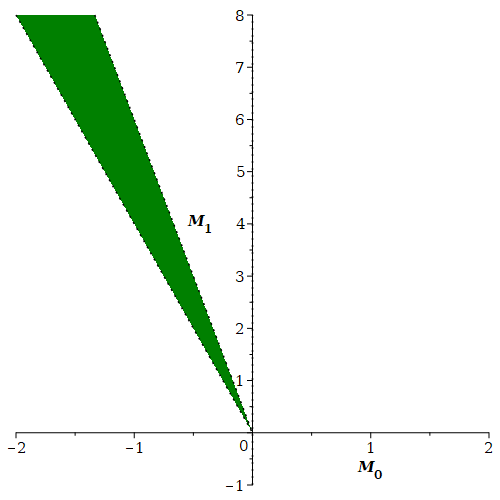
\includegraphics[width=6cm,trim={0 0 0 0},clip]{fig1.png} 
\caption{Acceptable values of \(M_{1}\) and \( M_{0}.\)}
\label{fig1}
\end{figure}

Wave profile (\ref{eq24}) at \(k=1.6,\, M_{0}=-1.48,\, M_{1}=6.16.\) is depicted on Fig. \ref{fig8}.
\begin{figure}[H]
\center
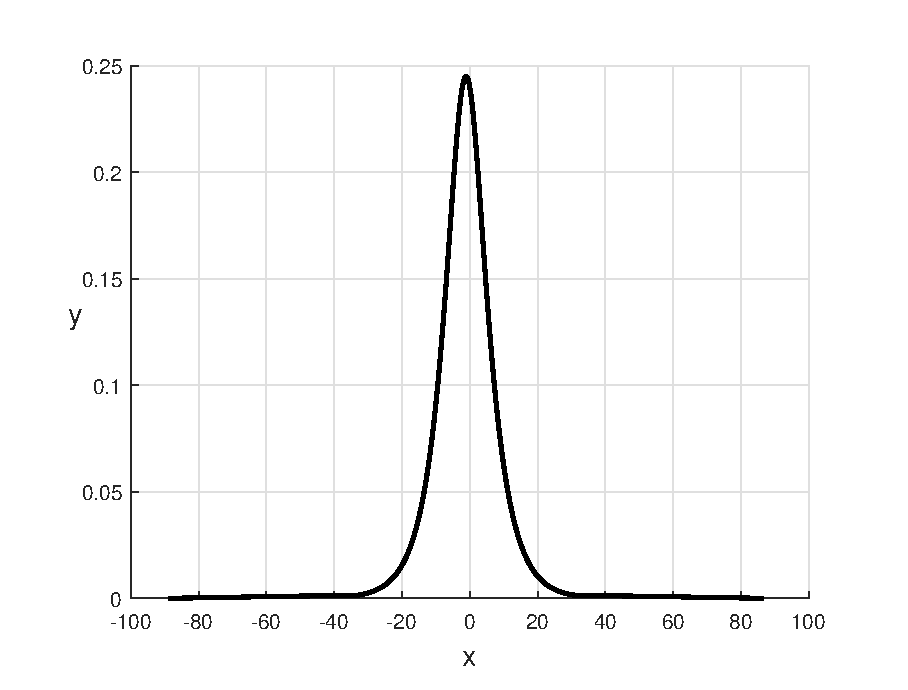
\includegraphics[width=0.5\linewidth]{fig10.eps}
\caption{Solitary wave prifile at \(k=1.6,\, M_{0}=-1.48,\, M_{1}=6.16.\)}
\label{fig8}
\end{figure}

\section{Modification of the split-step Fourier method for modeling processes described by cubic-quintic-septic nonlinear Schr\"{o}dinger equation}\label{ch3}

A family of generalized NLS equations can be written as follows:
\begin{equation}
u_{t}=i\mathscr{L} [u]+i\mathscr{N}[u]u,
\end{equation}
As example, at \(\mathscr{L} [u] \equiv a u_{xx},  \,\,  \mathscr{N} [u] \equiv b_{1} |u|^2\) we obtain the well-known nonlinear Shr\"{o}dinger equation (\ref{eq1}).

To implement a Fourier method, we denote a periodic boundary conditions, which yields:
\begin{equation} \label{eq30}
\begin{aligned}
\begin{cases}
u\left(-\frac{L}{2},t\right)=u\left(\frac{L}{2},t\right),\\
\cfrac{\partial u}{\partial x}\left(-\frac{L}{2},t\right)=\cfrac{\partial u}{\partial x}\left(\frac{L}{2},t\right).
\end{cases}
\end{aligned}
\end{equation}

Assuming \( x \in [-\frac{1}{2} L, \frac{1}{2} L]\), \( t \in [0, T]\), we divide x-interval in \(N\) equal parts with a spatial step
\begin{equation}
h=\frac{L}{N}.
\end{equation}

The space grid points are denoted as
\begin{equation}
x_{j}=jh, \quad j= -\frac{N}{2}, \ldots , \frac{N}{2}.
\end{equation}

Let \(\boldsymbol{U}^{m}\) be a grid approximation of a solution on a time layer \(m\) and \(\boldsymbol{V}^{m}\) be an interim solution. In this case, the initial conditions are set in \(\boldsymbol{U}^{0}\). In general, the split-step scheme can be written as follows\cite{Rad1}:
\begin{equation}\label{eq34}
\boldsymbol{U}^{m+1}=e^{i\tau\mathscr{L}}\boldsymbol{V}^m,
\end{equation}
where
\begin{equation}\label{eq33}
\boldsymbol{V}^m=e^{i\tau\mathscr{N}[\boldsymbol{U}^m]}\boldsymbol{U}^m.
\end{equation}

Applying the split-step Fourier method, it is proposed to use the discrete Fourier transform for the grid function \(\boldsymbol{V}^m\) to construct a solution on a next time layer:
\begin{equation} 
\hat{\boldsymbol{V}}^m=\frac{h}{L}\exp\left(-i \boldsymbol{\mu} \boldsymbol{x}^{T}\right)\cdot \boldsymbol{V}^{m},
\end{equation}
where \(\hat{\boldsymbol{V}}^m\) is the vector of Fourier coefficients, \(\boldsymbol{\mu}=\left(\mu_{-N/2},\ldots,\mu_{N/2-1}\right)^{T}\) is the transform frequency vector \(\mu_{n}=\frac{2\pi n}{L}\), \(\boldsymbol{x}=\left(x_{-N/2},\ldots,x_{N/2-1}\right)^{T}\) are the grid point coordinates.

There is a ratio between \(\hat{\boldsymbol{U}}^{m+1}\) and \(\hat{\boldsymbol{V}}^{m}\),
\begin{equation} \label{eq46}
\hat{\boldsymbol{U}}^{m+1}=\exp\left(-i \left(\boldsymbol{\mu}\circ \boldsymbol{\mu}\right) \tau\right)\circ \hat{\boldsymbol{V}}^{m},
\end{equation}
which is obtained by substituting a corresponding Fourier series for \(\boldsymbol{U}^{m+1}\) and \(\boldsymbol{V}^{m}\) in Eq. (\ref{eq34}). Here \(x\circ y\) refers to the Hadamard product.

The solution on the next time layer is found by the inverse Fourier transform using Eq. (\ref{eq46}):
\begin{equation} 
\boldsymbol{U}^{m+1}=\exp\left(i \boldsymbol{\mu} \boldsymbol{x}^{T}\right)\cdot \hat{\boldsymbol{U}}^{m+1}.
\end{equation}

Modifying the method for the Eq. (\ref{e4}), operators \(\mathscr{L} [u]\) and \(\mathscr{N}[u]\) take the form:
\begin{equation}
\begin{cases}
\mathscr{L} [u] \equiv u_{xx},  \\
\mathscr{N} [u] \equiv |u|^2+ \varepsilon_{2}|u|^4+ \varepsilon_{3}|u|^6.
\end{cases}
\end{equation}

A simplified flowchart for the numerical solution of the pulse propagation problem with periodic boundary conditions using the split-step Fourier method depicted on Fig. \ref{fig2}. 
\begin{figure}[H]
\begin{center}
\begin{minipage}[h]{0.48\linewidth} %% color here
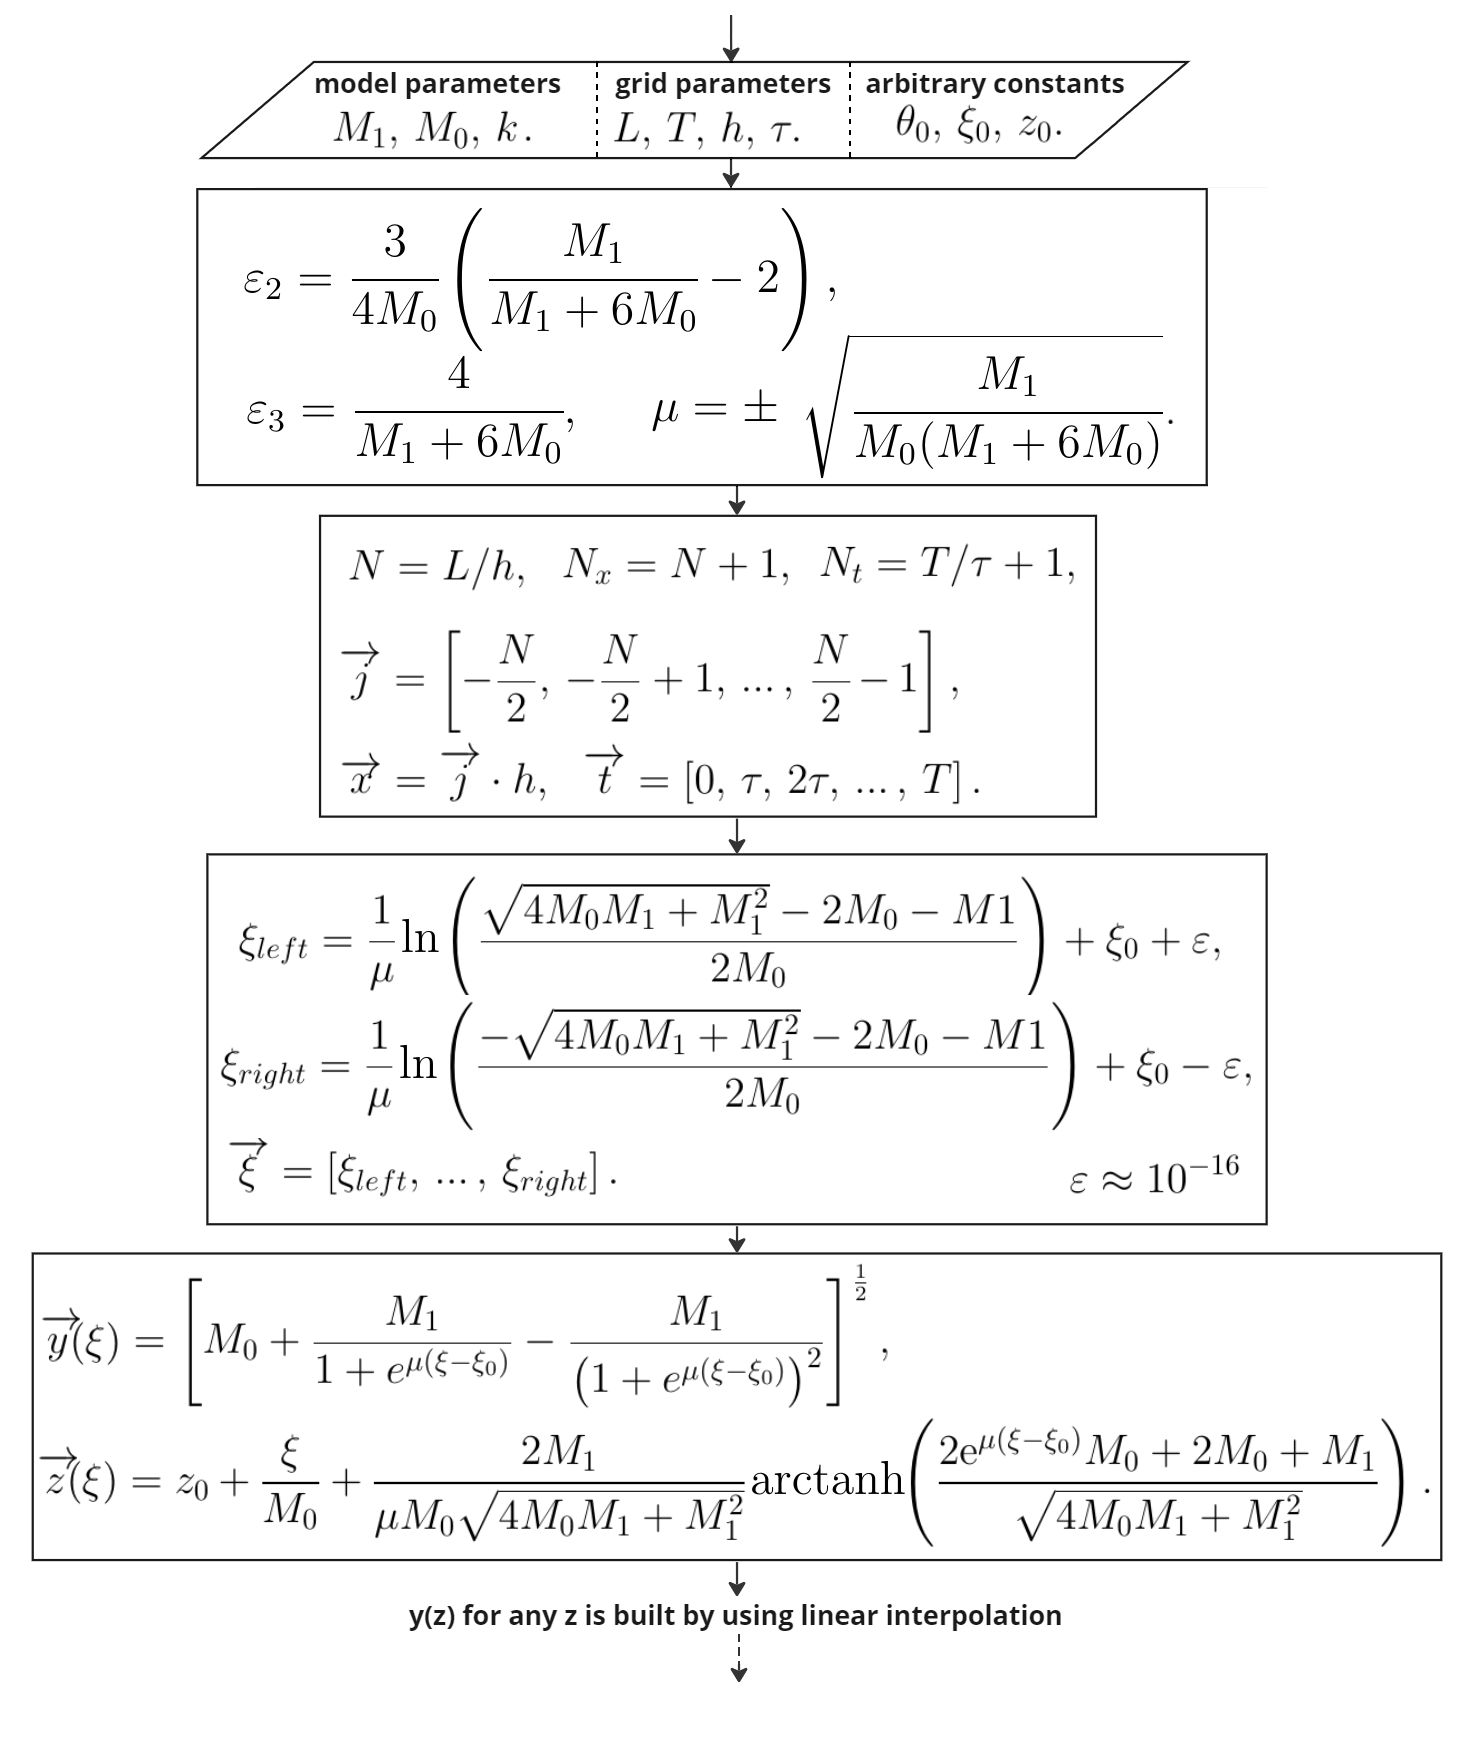
\includegraphics[width=1\linewidth]{fig2.png}
\end{minipage}
\hfill
\begin{minipage}[h]{0.48\linewidth}
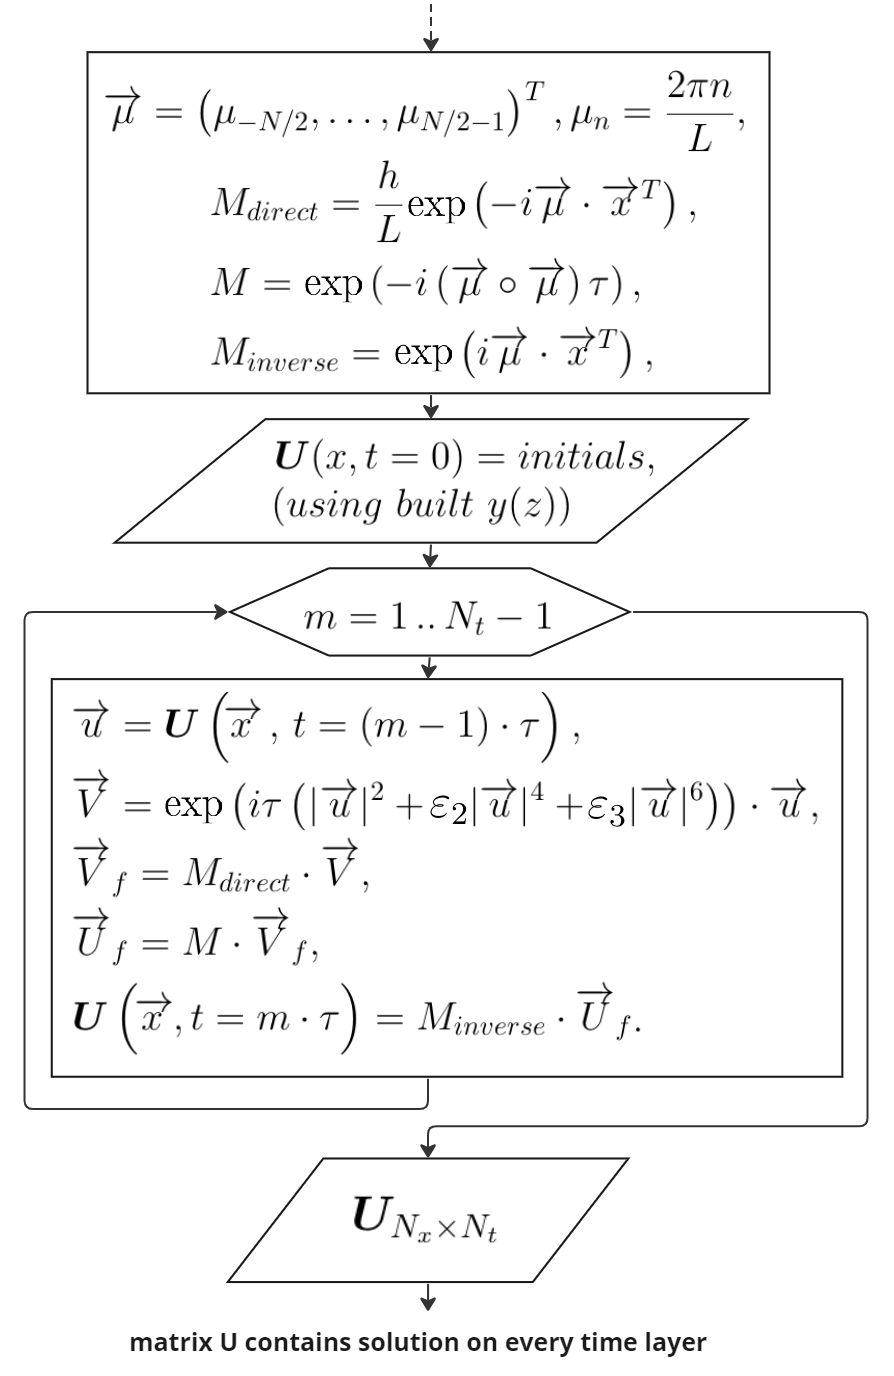
\includegraphics[width=0.75\linewidth]{fig3.png}
\end{minipage}
\end{center}
\caption{Flowchart for modeling the pulse propagation process using the Fourier method.}
\label{fig2}
\end{figure}

\section{Application of the Fourier method for modeling pulse propagation process described by the cubic-quintic-septic nonlinear Schr\"{o}dinger equation}\label{ch6}
Let us consider Eq. (\ref{e4}). To verify the analytical calculations, we numerically simulate the process of propagation of a solitary wave (\ref{eq24}). We perform a computation for certain parameters \(M_{0}\) and \(M_{1}\), fulfilling the constraints (\ref{eq27}). Parameters \(\varepsilon_{1}\),\,\(\varepsilon_{2}\),\,\(\omega\) and \(\mu\) are determined by formulas (\ref{eq19}). The result of the modeling are depicted on Fig.\ref{fig10}. Analytical and numerical profiles at the moment \(t=16\) are depicted in Fig. \ref{fig10a}.

\begin{figure}[H]
\begin{center}
\begin{minipage}[h]{0.48\linewidth} %% color here
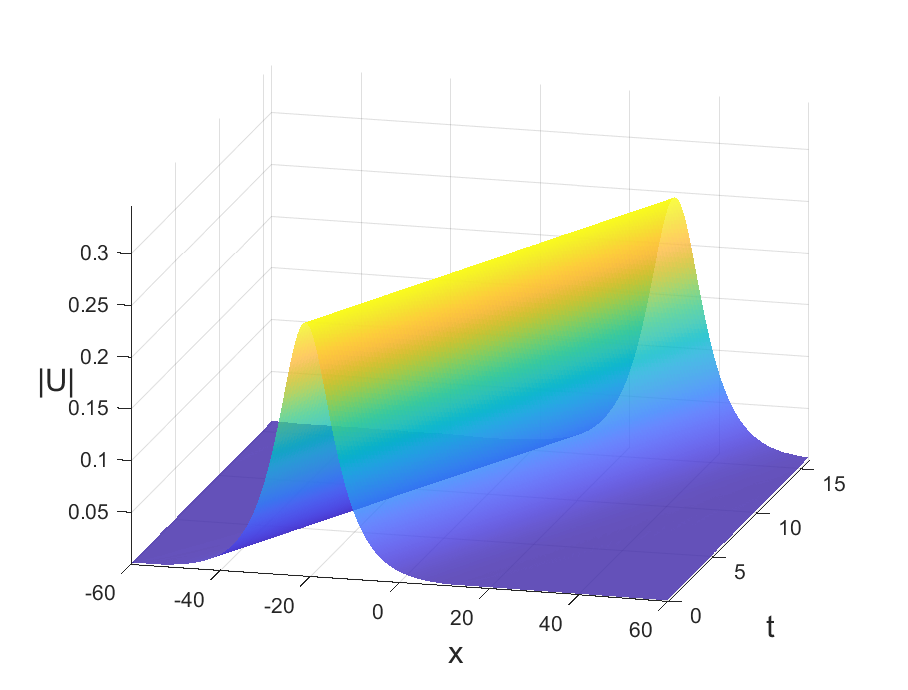
\includegraphics[width=1\linewidth]{fig11.eps}
\subcaption{Numerical solution surface plot} 
\label{fig10a}
\end{minipage}
\hfill
\begin{minipage}[h]{0.48\linewidth}
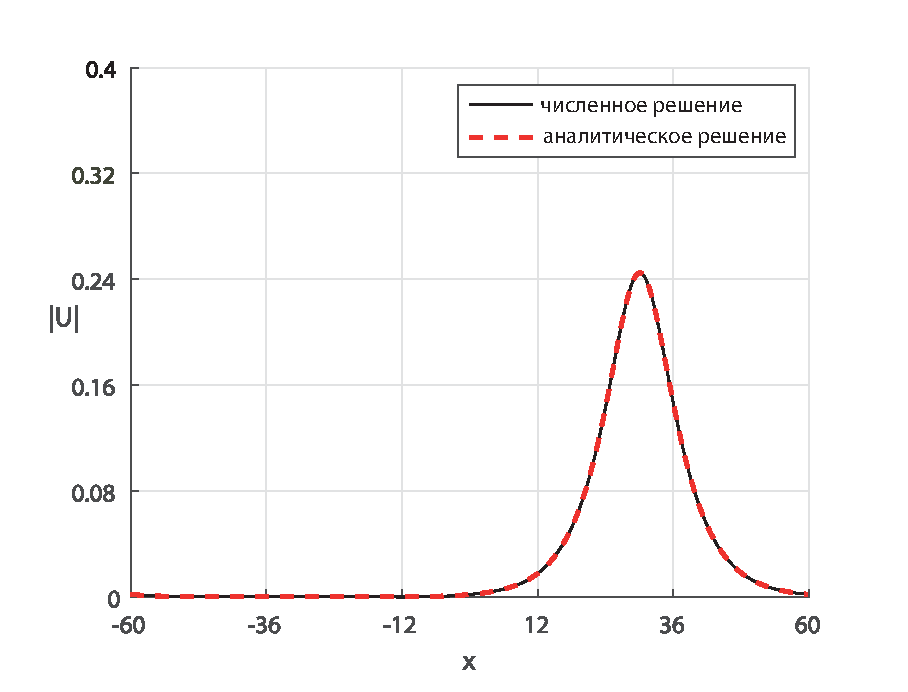
\includegraphics[width=1\linewidth]{fig12.eps}
\subcaption{Solution module at t=16}
\label{fig10b}
\end{minipage}
\end{center}
\caption{Propagation of a solitary wave (\ref{eq24}) \\
at the parameters
\(L=120,\, T=16,\, h=0.2,\, \tau=0.04\), 
\(z_{0}=-20,\,k=1.6,\, M_{0}=-1.48,\, M_{1}=6.16\).}
\label{fig10}
\end{figure}
The relative error for calculation at the specified parameters does not exceed 0.08\%.  The dependence of a relative error over time is illustrated in Fig. \ref{fig11a}.

\begin{figure}[H]
\begin{center}
\begin{minipage}[h]{0.48\linewidth} %% color here
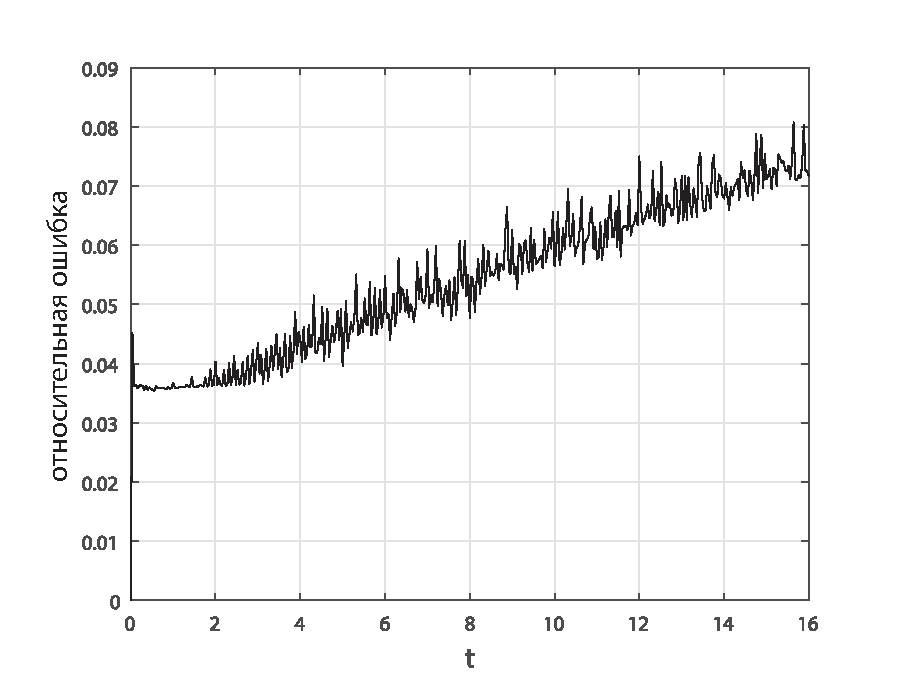
\includegraphics[width=1\linewidth]{fig13.eps}
\subcaption{Relative error over time at \(h=0.2,\, \tau=0.04\)} 
\label{fig11a}
\end{minipage}
\hfill
\begin{minipage}[h]{0.48\linewidth}
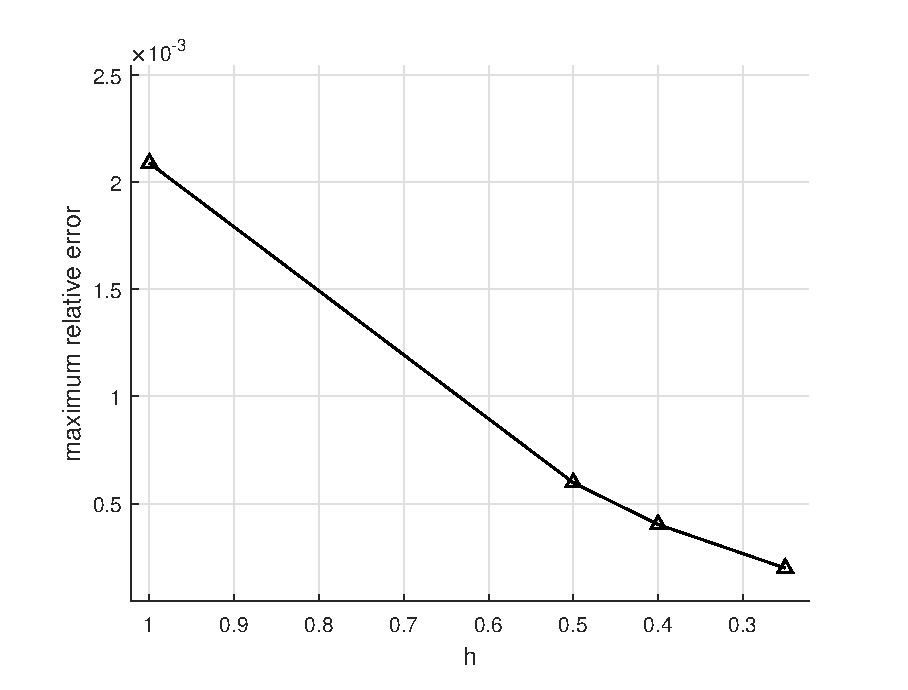
\includegraphics[width=1\linewidth]{fig45.eps}
\subcaption{Maximum relative error over grid space step \(h\)}
\label{fig11b}
\end{minipage}
\end{center}
\caption{Numerical results at the parameters
\(L=120,\, T=16\), 
\(M_{0}=-1.48,\, M_{1}=6.16\).}
\label{fig11}
\end{figure}
Since grid convergence is achieved (see Fig. \ref{fig11b}), we claim that all analytical calculations are correct. Hence, we conclude that the analytical solution built in Section \ref{ch2} describe a stable soliton which can be used for signal transmission.

\section{Interaction of soliton with perturbation in initial conditions}\label{ch8}
Let us consider a numerical modeling of the pulse propagation at initial perturbation. We disturb the initial condition, corresponding to solution (\ref{eq24}) of Eq. (\ref{e4}) in the following way:
\begin{equation} \label{eq52}
u(x,0)=y\left(\xi\left(x\right)\right)\cdot e^{i(kx-\theta_{0})}+Ae^{-\nu(x-x_{0})^{2}}.
\end{equation}
The corresponding numerical solutions are depicted in Fig. \ref{fig17}.
\begin{figure}[H] %% color here
\begin{center}
\begin{minipage}[h]{0.48\linewidth}
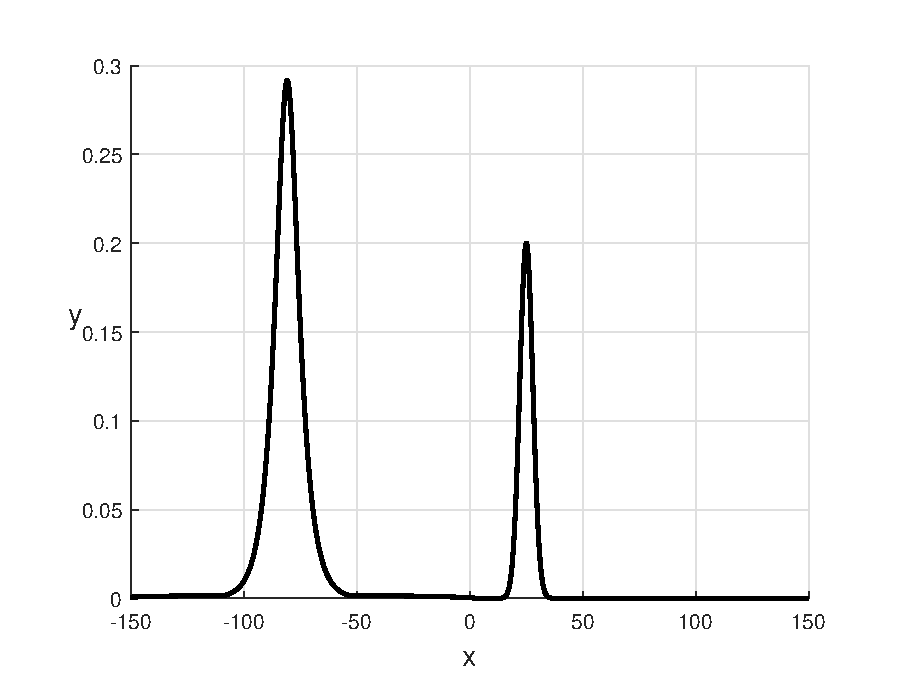
\includegraphics[width=1\linewidth]{fig18.eps}
\subcaption{Module of initial profile (\ref{eq52}) }
\end{minipage}
\hfill
\begin{minipage}[h]{0.48\linewidth}
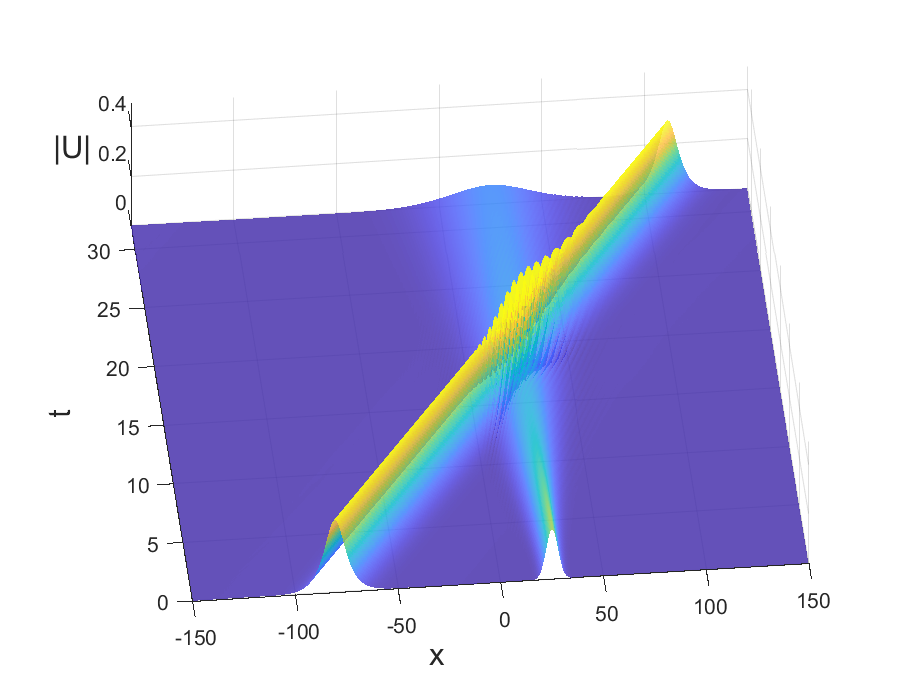
\includegraphics[width=1\linewidth]{fig19.eps}
\subcaption{Module of numerical solution}
\end{minipage}
\end{center}
\caption{Plots of numerical results at the parameters \(M_{0}=-3,\,M_{1}=12.34,\, k=3,\, \xi_{0}=0,\,z_{0}=-80,\, \theta_{0}=0\), \\
\(L=300,\, T=32,\, h=0.25,\, \tau=0.625,\,A=0.2,\,\nu=0.06,\, x_{0}=25\).}
\label{fig17}
\end{figure}
This simulation allows us to conclude that the soliton specified by the parameters \(M_{0}=-3,\,M_{1}=12.34\), interacts with the given perturbation and does not lose the ability to propagate. The pulse profile is restored after interaction.

It is found that the soliton (\ref{e4}) is stable when propagating in a medium with random noise of the following type:
\begin{equation} \label{eq522}
u(x,0)=y\left(\xi\left(x\right)\right)\cdot e^{i(kx-\theta_{0})}+A\cdot rand(x).
\end{equation}
The corresponding illustrations are depicted in Fig. \ref{fig172}.	
\begin{figure}[H] %% color here
\begin{center}
\begin{minipage}[h]{0.48\linewidth}
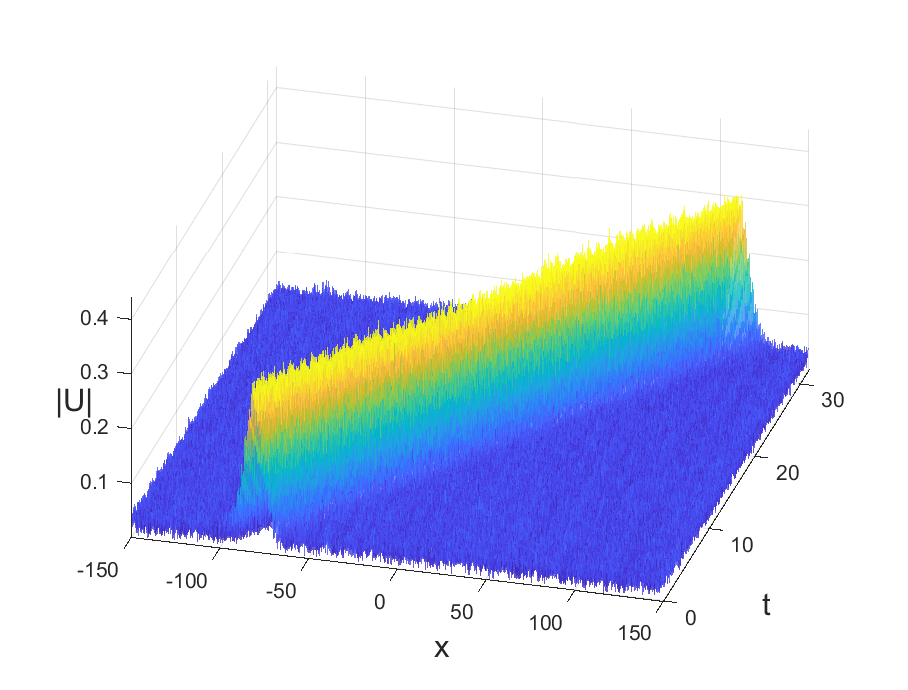
\includegraphics[width=1\linewidth]{fig46.eps}
\subcaption{Module of numerical solution}
\end{minipage}
\hfill
\begin{minipage}[h]{0.48\linewidth}
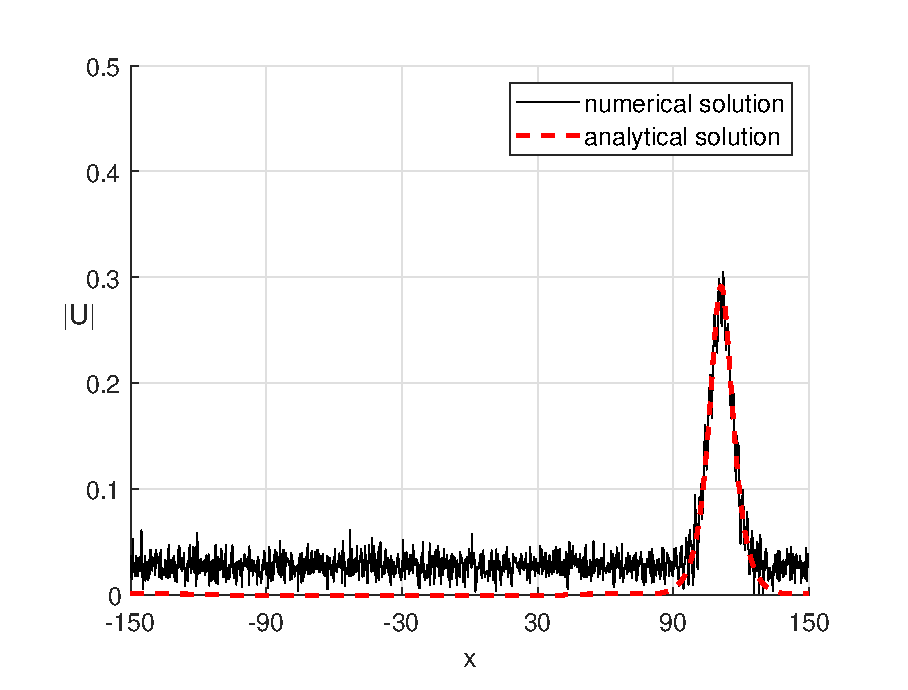
\includegraphics[width=1\linewidth]{fig47.eps}
\subcaption{Wave profiles at t=32}
\end{minipage}
\end{center}
\caption{Plots of numerical results at the parameters \(M_{0}=-3,\,M_{1}=12.34,\, k=3,\, \xi_{0}=0,\,z_{0}=-80,\, \theta_{0}=0\), \\
\(L=300,\, T=32,\, h=0.25,\, \tau=0.0625,\,A=0.05\).}
\label{fig172}
\end{figure}

The simulations carried out in this section confirm the stability of the solitons obtained in Section \ref{ch2}.
\section{Analysis of the higher-power nonlinearities influence on the solitary wave propagation}\label{ch9}
In many physical applications, some pertirbation terms are introduced into NLS equation. In a mathematical model, it is not always possible to take them into account in advance. In this section we investigate the impact of the additional nonlinear terms on the solutions of the NLS equation.

At \(\varepsilon_{2}=0,\,\varepsilon_{3}=0\), the Eq. (\ref{e4}) takes the form:
\begin{equation}\label{e6}
iu_{t}+u_{xx}+|u|^2 u=0.
\end{equation}
This well-known NLS equation is completely integrable. The solution of Eq. (\ref{e6}) in the form of a solitary wave has been found in paper \cite{Rad3} and takes the following form:
\begin{equation} \label{eq48}
u(x,t)=\frac{4(k^{2}-\omega)}{2 (k^{2}-\omega) e^{-\left(x-c_{0}t-z_{0}\right)\sqrt{(k^{2}-\omega)}}+e^{\left(x-c_{0}t-z_{0}\right)\sqrt{(k^{2}-\omega)}}}\cdot e^{i(kx-\omega t-\theta_{0})},
\end{equation}
where \(c_{0}=2k\) and \( k,\, \omega,\, z_{0},\, \theta_{0}\) are arbitrary constants.
The initial condition corresponding to Eq. (\ref{eq48}) takes the form:
\begin{equation}\label{eq55}
u(x,0)=\frac{4\,(k^{2}-\omega)}{2 (k^{2}-\omega) e^{-(x-z_{0})\sqrt{(k^{2}-\omega)}}+e^{(x-z_{0})\sqrt{(k^{2}-\omega)}}}\cdot e^{i(kx-\theta_{0})}
\end{equation}

At \(\varepsilon_{3}=0\), the solution of the Eq. (\ref{e4}) was found and takes following the form:
\begin{equation}\label{e7}
u(x,t)=\left(\frac{4\,\mu\, e^{\sqrt{\mu}\,(x-2kt-z_{0})}}{1+4\, e^{\sqrt{\mu}\,(x-2kt-z_{0})}+(4+4\, \mu\, \nu) \,e^{2\sqrt{\mu}\,(x-2kt-z_{0})}}\right)^{\frac{1}{2}}\cdot e^{i(kx-\omega t-\theta_{0})},
\end{equation}
where \(\mu=4(\omega-k^{2})\), \(\nu=\cfrac{4 \varepsilon_{2}}{3}\) and \( k,\, \omega,\, z_{0},\, \theta_{0}\) are arbitrary constants. We note that at \(\varepsilon_{2}=0\) Eq. (\ref{e7}) coincides with Eq. (\ref{eq48}).

Let us consider how the behavior of a solitary wave Eq. (\ref{eq55}) is affected by the presence of higher nonlinearity terms.
We consider the physical process described by the Eq. (\ref{e4}) and assume that the parameters \(\varepsilon_{2}\) and \(\varepsilon_{3}\) are neglected when setting up the initial pulse.

In the absence of the highest nonlinear powers at \(\varepsilon_{2}=0,\,\varepsilon_{3}=0\) the solitary wave (\ref{eq48}) is the exact solution of the Eq. (\ref{e4}). The numerical solution for the initial pulse (\ref{eq55}) coincides with the analytical.

When the nonlinearity parameter \(\varepsilon_{2}\ne 0\) is taken into account, the decay of the initial pulse is observed. Decay is accompanied by soliton oscillations and energy emission. It is observed that the soliton (\ref{eq55}), when oscillating and emitting energy, transforms into a stable soliton solution coinciding with the Eq. (\ref{e7}). The simulation result is illustrated in Fig. \ref{fig21_1} and \ref{fig21_2}.
\begin{figure}[H] %% color here
\begin{center}
\begin{minipage}[h]{0.48\linewidth}
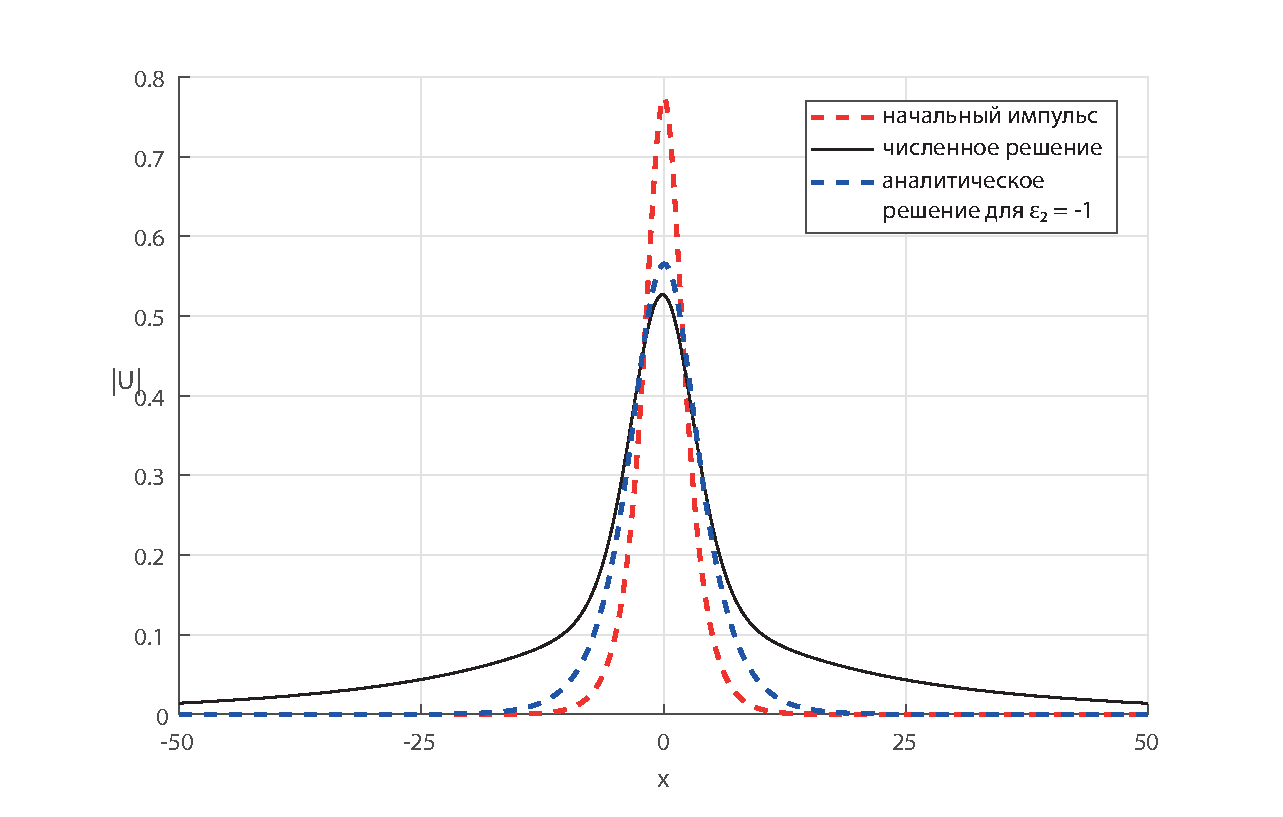
\includegraphics[width=1\linewidth]{fig33.eps}
\subcaption{Solution profile at t=25}
\end{minipage}
\hfill
\begin{minipage}[h]{0.48\linewidth}
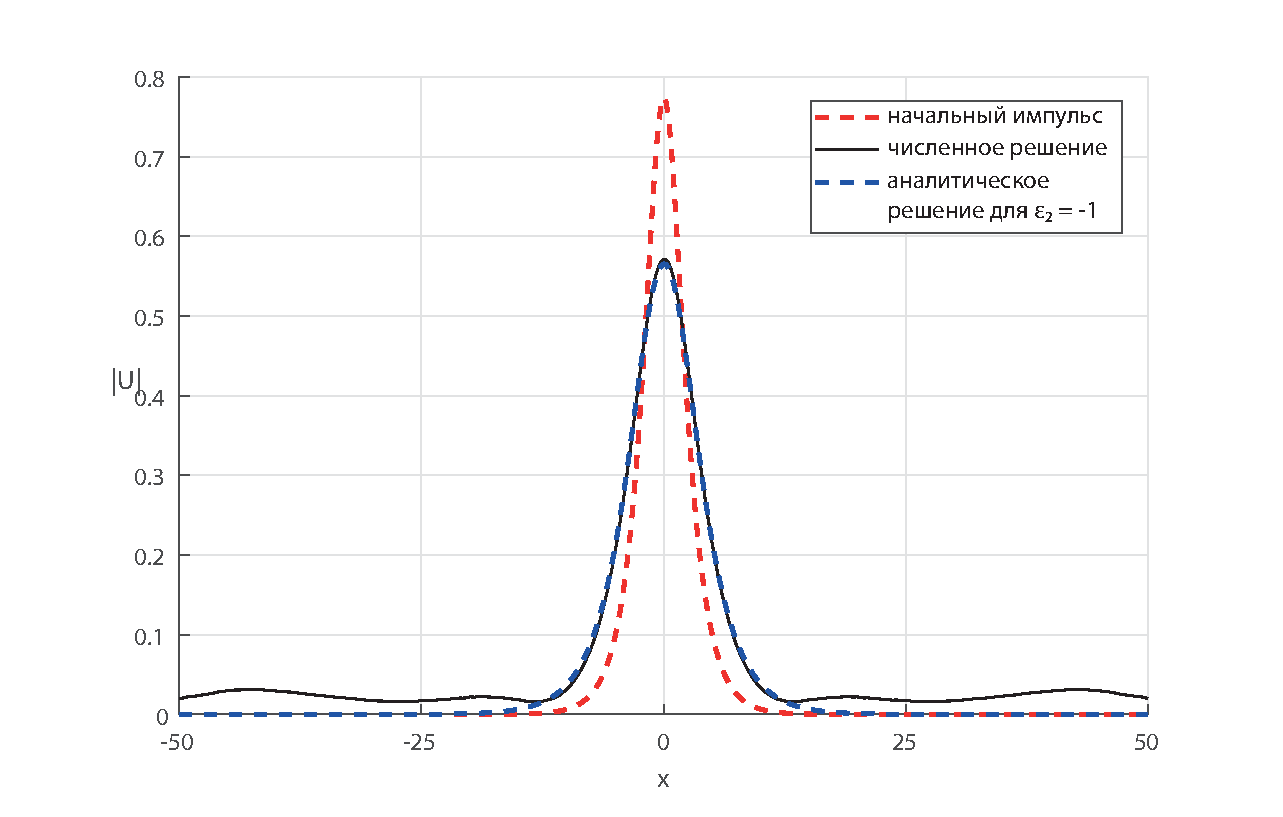
\includegraphics[width=1\linewidth]{fig34.eps}
\subcaption{Solution profile at t=200}
\end{minipage}
\end{center}
\caption{Results for the initial pulse (\ref{eq55}) at
\(L=200,\, T=200,\, h=0.25,\, \tau=0.0625,\)
\(\varepsilon_{2}=-1,\,\varepsilon_{3}=0,\, \omega=0.2,\, k=0.707\).}
\label{fig21_1}
\end{figure}

Relative error between analytical solution (\ref{e7}) and numerical solution over time is illustrated in Fig. \ref{fig21_2a}. 
\begin{figure}[H]
\begin{center}
\begin{minipage}[h]{0.48\linewidth}
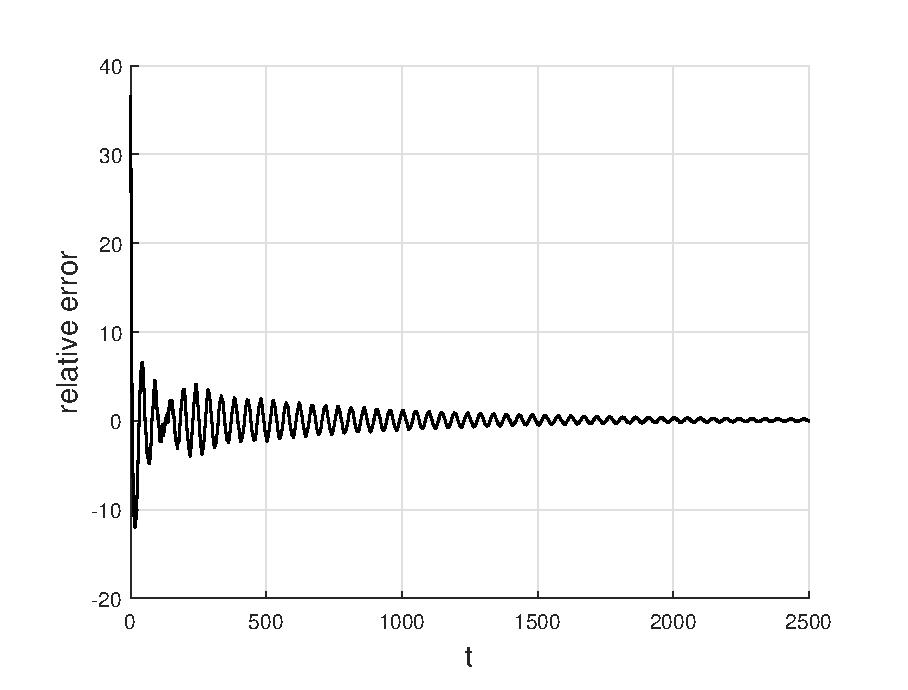
\includegraphics[width=1\linewidth]{fig48.eps}
\subcaption{Relative error over time}
\label{fig21_2a}
\end{minipage}
\hfill
\begin{minipage}[h]{0.48\linewidth}
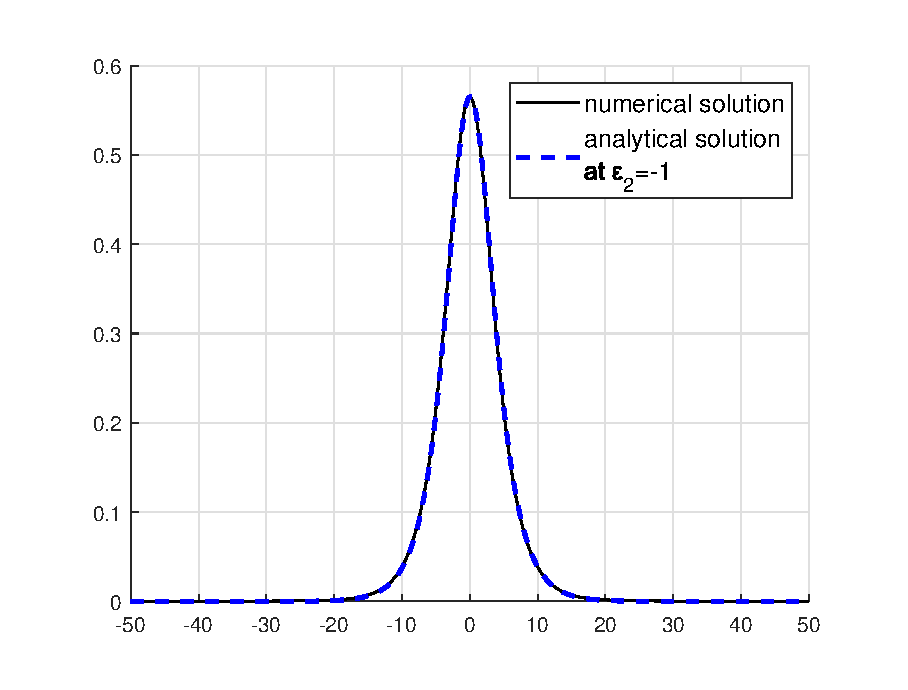
\includegraphics[width=1\linewidth]{fig49.eps}
\subcaption{Solution profile at t=2500}
\label{fig21_2b}
\end{minipage}
\end{center}
\caption{Results for the initial pulse (\ref{eq55}) at
\(L=200,\, T=200,\, h=0.25,\, \tau=0.0625,\)
\(\varepsilon_{2}=-1,\,\varepsilon_{3}=0,\, \omega=0.2,\, k=0.707\).}
\label{fig21_2}
\end{figure}

When the highest power is taken into account at \(\varepsilon_{3}\ne0\), oscillatory behavior persists. It is found that the sign of the \(\varepsilon_{3}\) affects the damping rate of oscillations. At \(\varepsilon _{3}<0\) the damping is more intense and the amplitude of the stable pulse is reduce. At \(\varepsilon _{3}>0\) the oscillations stop at longer times with increased stable pulse amplitude. The illustrations of the pulse amplitude behavior are depicted in Fig. \ref{fig48}. Here the parameter \(\delta\) is the relative size of the oscillations gap.
\begin{figure}[H] %% color here
\begin{minipage}[h]{1\linewidth}
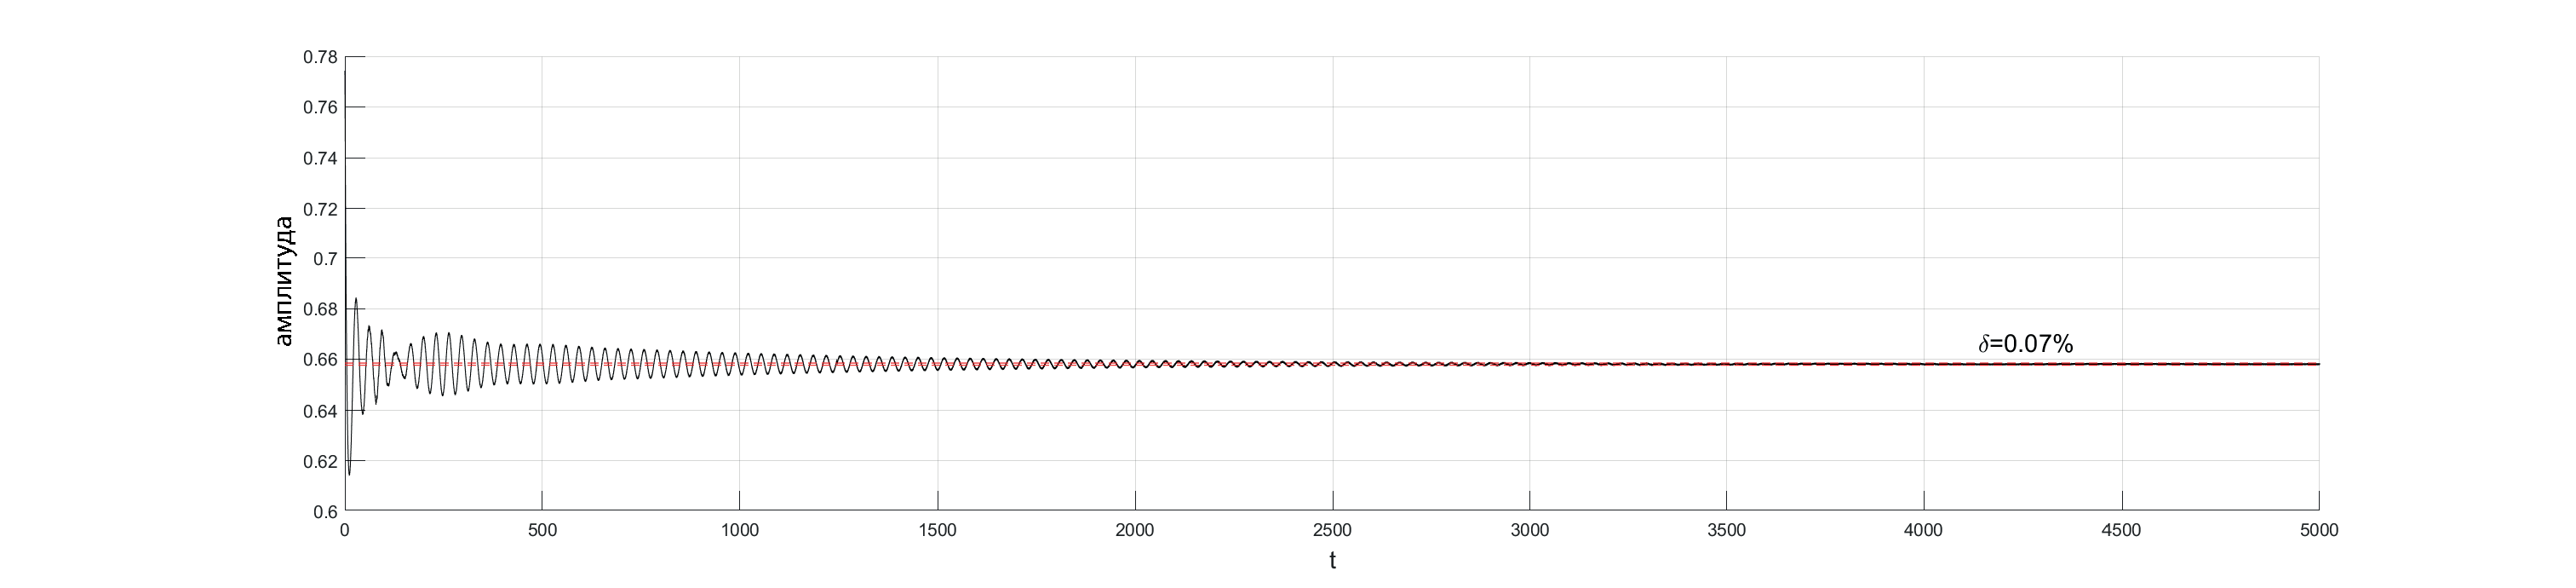
\includegraphics[width=1\linewidth]{fig35.eps}
\subcaption{\(\varepsilon_{2}=-0.5,\,\varepsilon_{3}=0\)}
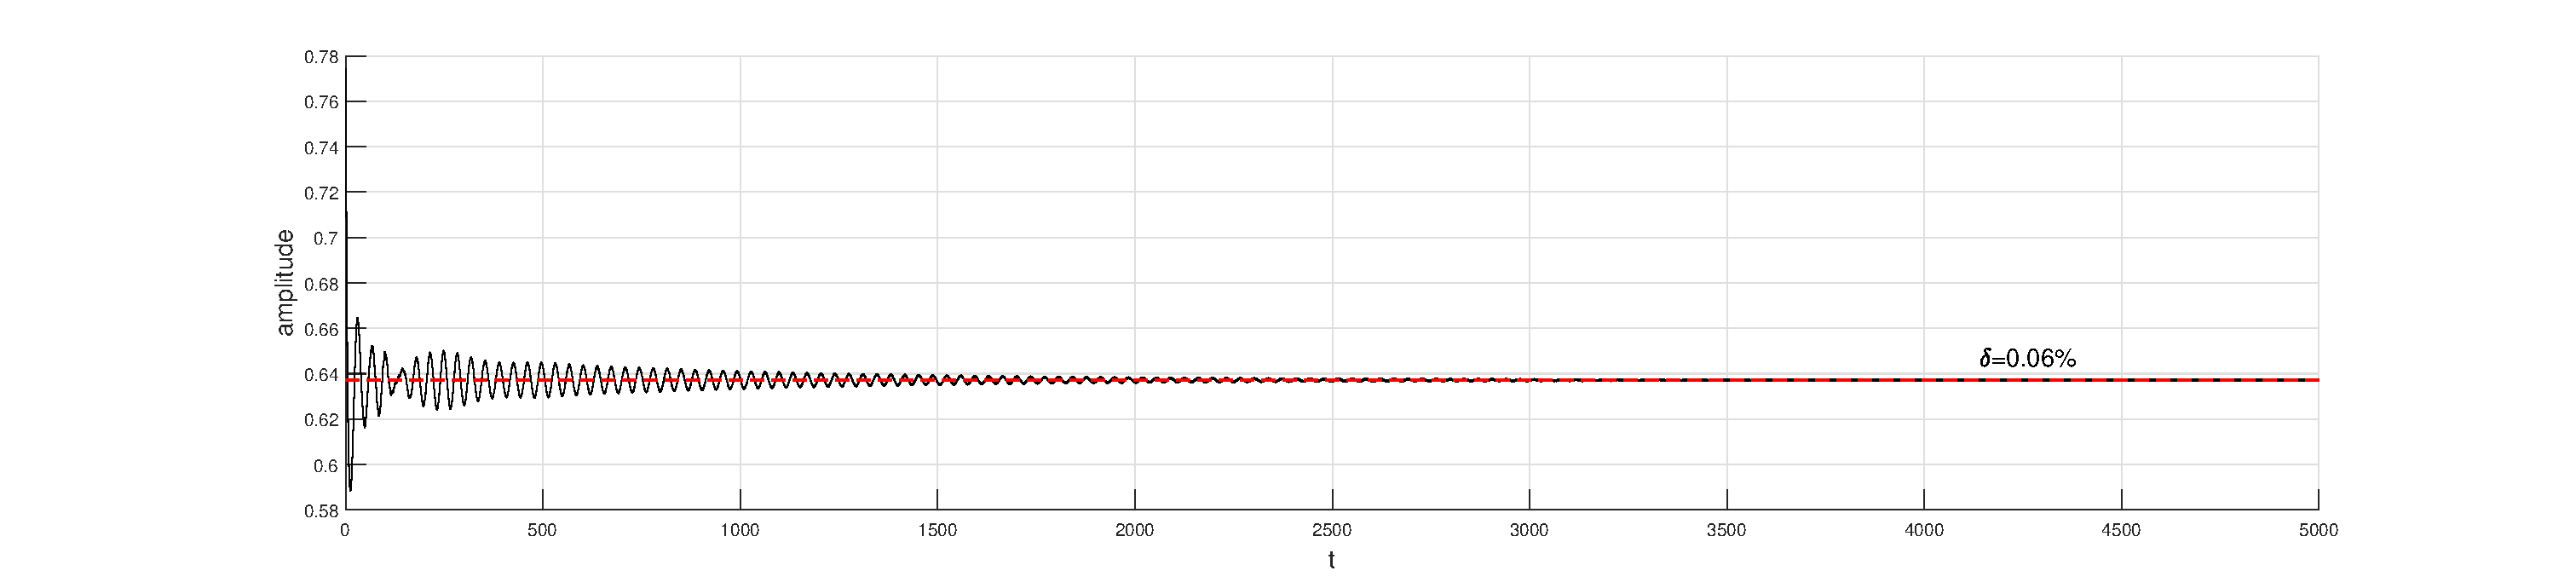
\includegraphics[width=1\linewidth]{fig36.eps}
\subcaption{\(\varepsilon_{2}=-0.5,\,\varepsilon_{3}=-0.25\)}
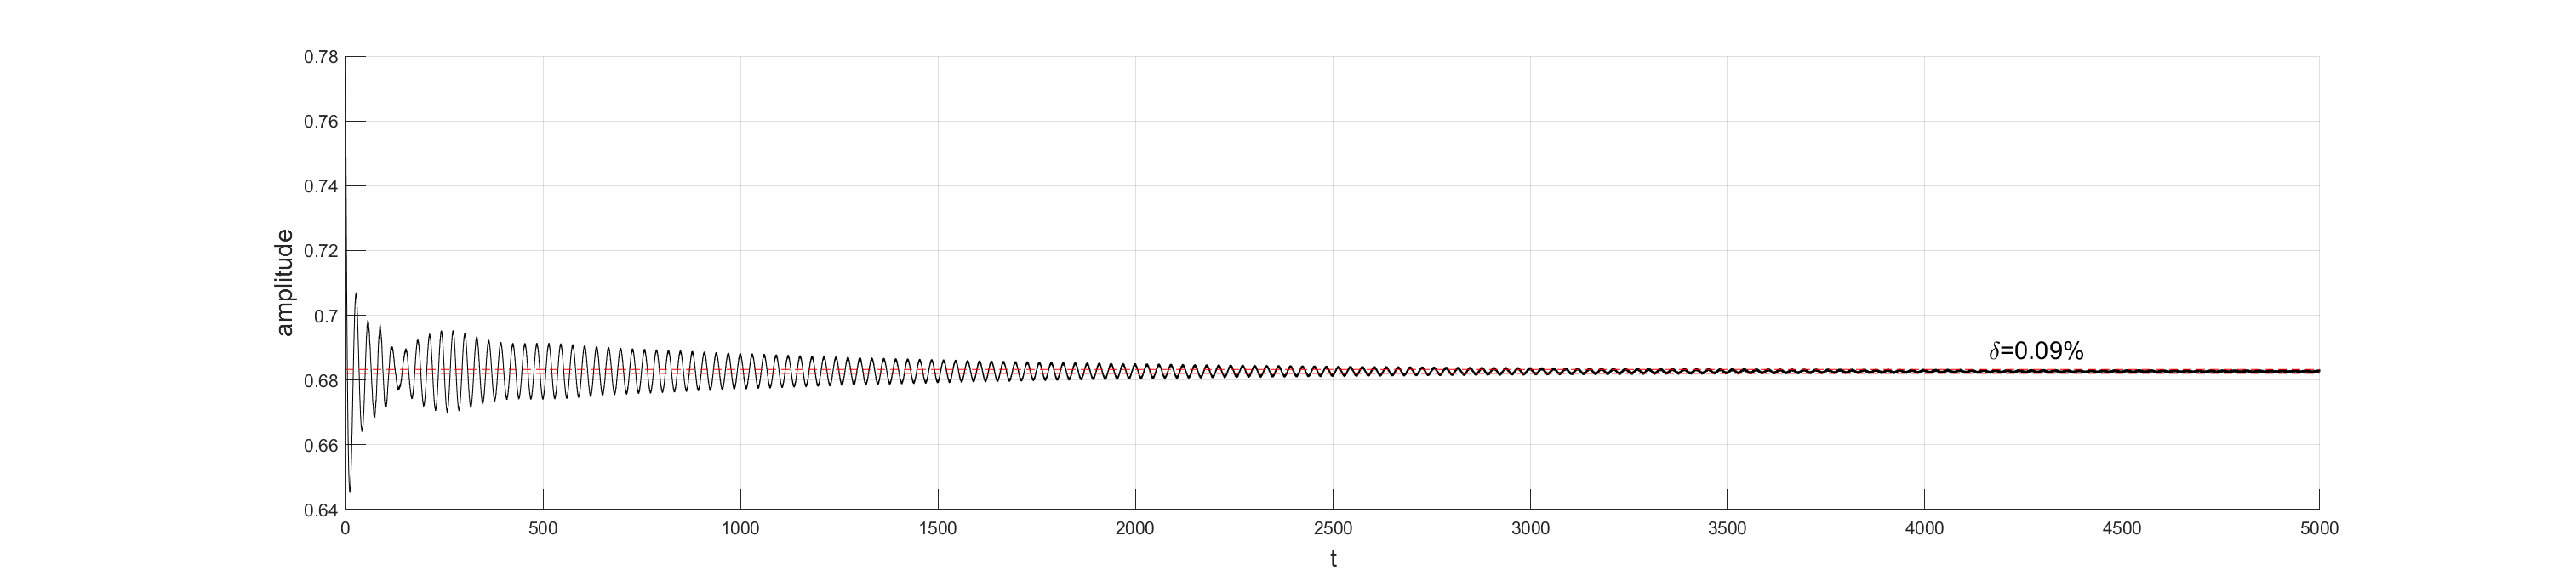
\includegraphics[width=1\linewidth]{fig37.eps}
\subcaption{\(\varepsilon_{2}=-0.5,\,\varepsilon_{3}=0.25\)}
\end{minipage}
\caption{The behavior of the pulse (\ref{eq55}) amplitude in the presence of the highest nonlinearities.
\(L=200,\, T=5000,\, h=0.25,\, \tau=0.0625,\, \omega=0.2,\, k=0.707\).}
\label{fig48}
\end{figure}

We conclude that the solitary waves of the NLS equation when propagating in a medium with higher nonlinear terms, are transformed into stable solitons of a generalized non-integrable model. This transition is accompanied by the energy emission and oscillations of the initial pulse. It is found that the addition of a 7th power nonlinear term affects the rate of transformation into a stable soliton. The sign of \(\varepsilon_{3}\) affects the duration of the oscillations and the amplitude of the stable impulse.

\section{Soliton collisions in the presence of higher nonlinearity terms}\label{ch10}
The solutions of a completely integrable nonlinear Schr\"{o}dinger equation interact elastically, i.e. without momentum and energy exchange. When the integrability of the system is violated by external perturbations, soliton collisions become inelastic. In this section we investigate the NLS equation soliton collisions in a medium, which is perturbed by nonlinear terms according to the Eq. (\ref{e4}).

Let us consider the collision of two solitons of the form (\ref{eq55}) with the parameters \(k_{1},\,k_{2},\,\omega_{1},\,\omega_{2},\,z_{0,1},\,z_{0,2},\,\theta_{0,1},\,\theta_{0,2}\). The value of the parameters \(\varepsilon_{2}\) and \(\varepsilon_{3}\) affects the intensity of energy and momentum exchange. It is found that the type of interaction depends on the solitons initial phase detunnung \(\Delta \theta=\theta_{0,1}-\theta_{0,2}\).

Simulation results at \(k_{1}=-k_{2},\,\omega_{1}=\omega_{2},\,z_{0,1}=-z_{0,2},\,\theta_{0,1}=\theta_{0,2}+Delta \theta\) are illustrated in Fig. \ref{fig50} and Fig. \ref{fig51}.

\begin{figure}[H]
\begin{minipage}[h]{0.32\linewidth}
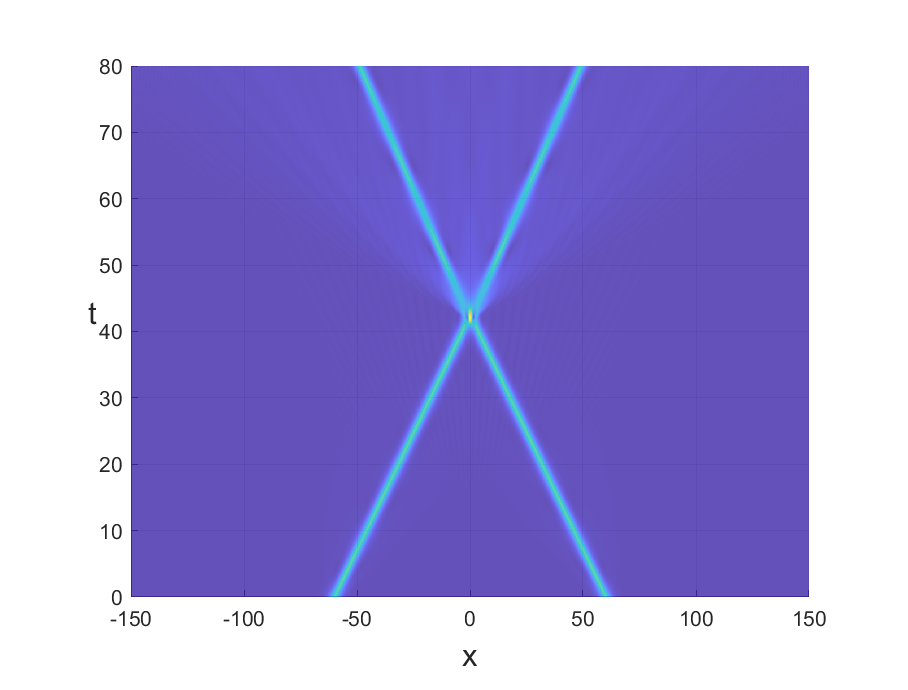
\includegraphics[width=1\linewidth]{fig52.eps}
\subcaption{\(\Delta \theta=0,\)\\\( \varepsilon_{2}=0.2,\,\varepsilon_{3}=-0.1\)}
\end{minipage}
\begin{minipage}[h]{0.32\linewidth}
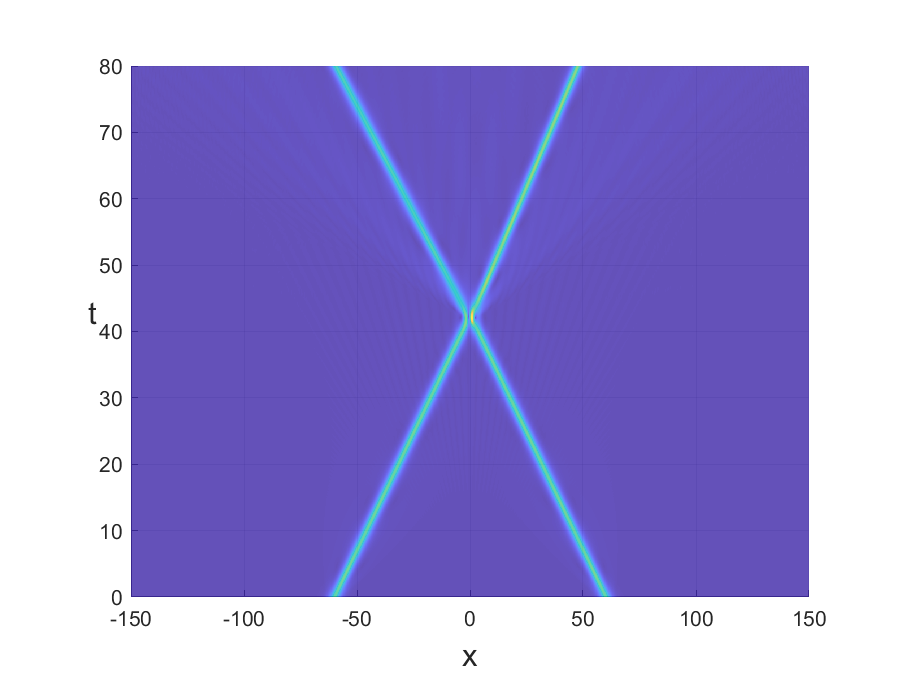
\includegraphics[width=1\linewidth]{fig55.eps}
\subcaption{\(\Delta \theta=\frac{\pi}{2},\)\\\( \varepsilon_{2}=0.2,\,\varepsilon_{3}=-0.1\)}
\end{minipage}
\begin{minipage}[h]{0.32\linewidth}
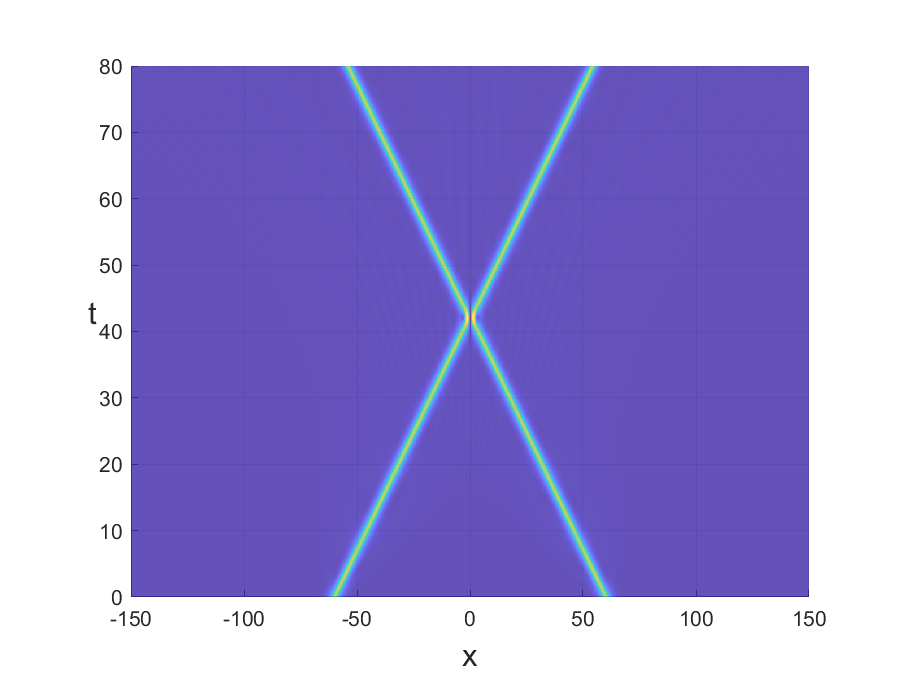
\includegraphics[width=1\linewidth]{fig58.eps}
\subcaption{\(\Delta \theta=\pi,\)\\\( \varepsilon_{2}=0.2,\,\varepsilon_{3}=-0.1\)}
\end{minipage}

\begin{minipage}[h]{0.32\linewidth}
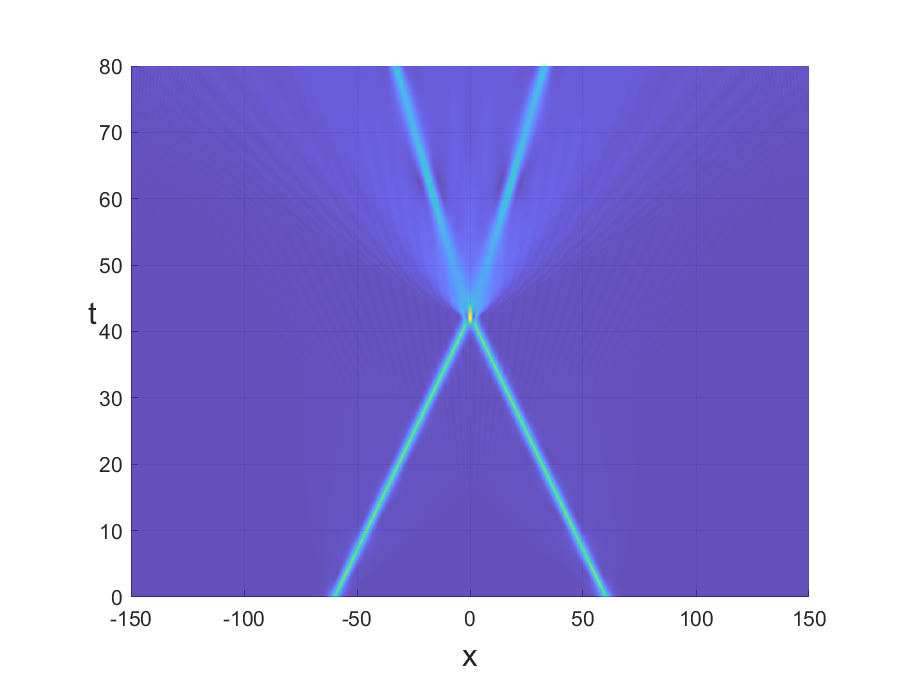
\includegraphics[width=1\linewidth]{fig53.eps}
\subcaption{\(\Delta \theta=0,\)\\\( \varepsilon_{2}=0.4,\,\varepsilon_{3}=-0.2\)}
\end{minipage}
\begin{minipage}[h]{0.32\linewidth}
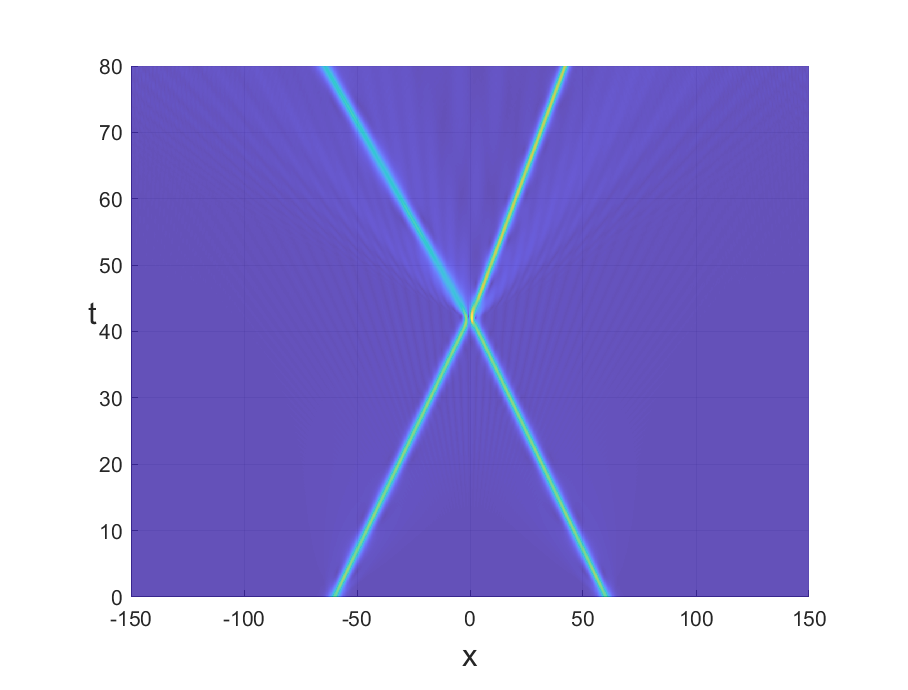
\includegraphics[width=1\linewidth]{fig56.eps}
\subcaption{\(\Delta \theta=\frac{\pi}{2},\)\\\( \varepsilon_{2}=0.4,\,\varepsilon_{3}=-0.2\)}
\end{minipage}
\begin{minipage}[h]{0.32\linewidth}
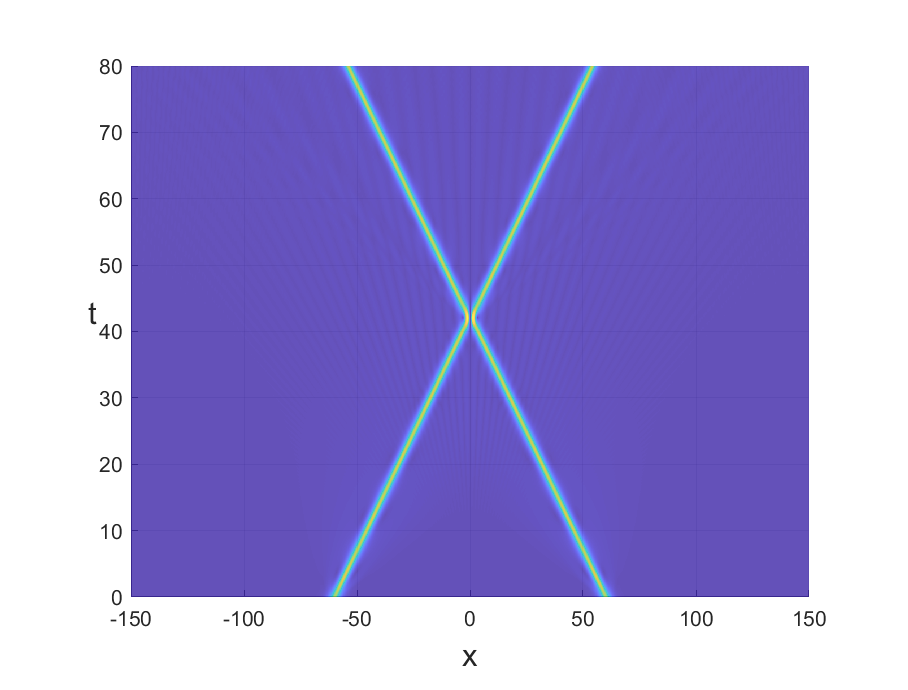
\includegraphics[width=1\linewidth]{fig59.eps}
\subcaption{\(\Delta \theta=\pi,\)\\\( \varepsilon_{2}=0.4,\,\varepsilon_{3}=-0.2\)}
\end{minipage}

\begin{minipage}[h]{0.32\linewidth}
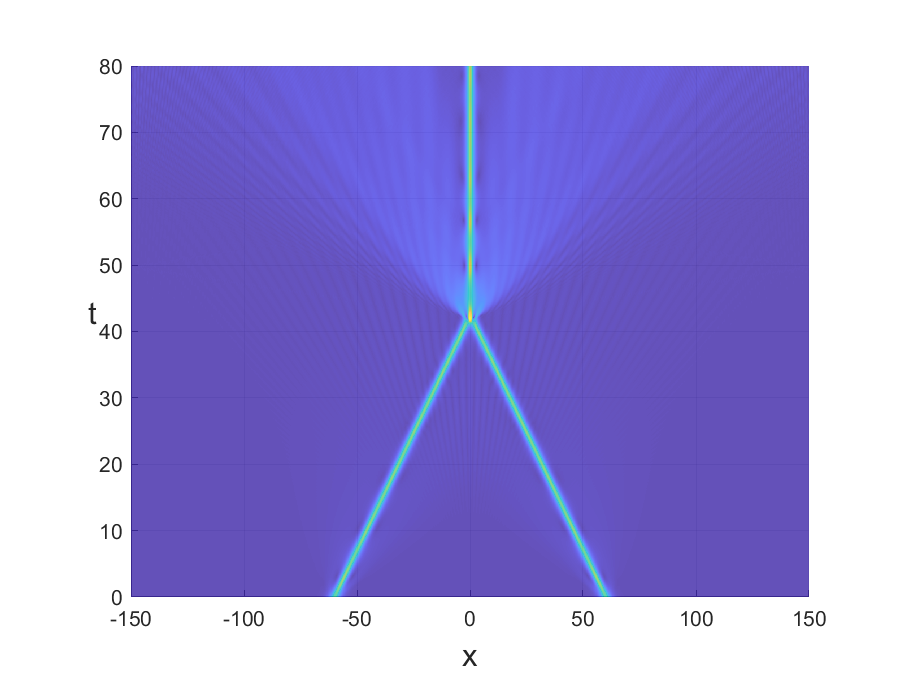
\includegraphics[width=1\linewidth]{fig54.eps}
\subcaption{\(\Delta \theta=0,\)\\\( \varepsilon_{2}=0.6,\,\varepsilon_{3}=-0.3\)}
\end{minipage}
\begin{minipage}[h]{0.32\linewidth}
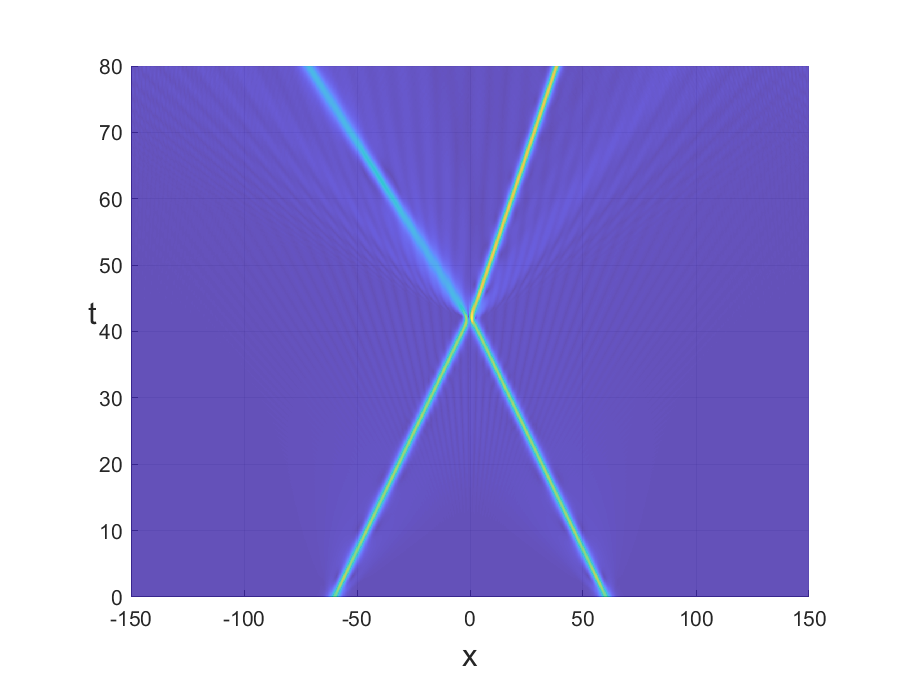
\includegraphics[width=1\linewidth]{fig57.eps}
\subcaption{\(\Delta \theta=\frac{\pi}{2},\)\\\( \varepsilon_{2}=0.6,\,\varepsilon_{3}=-0.3\)}
\end{minipage}
\begin{minipage}[h]{0.32\linewidth}
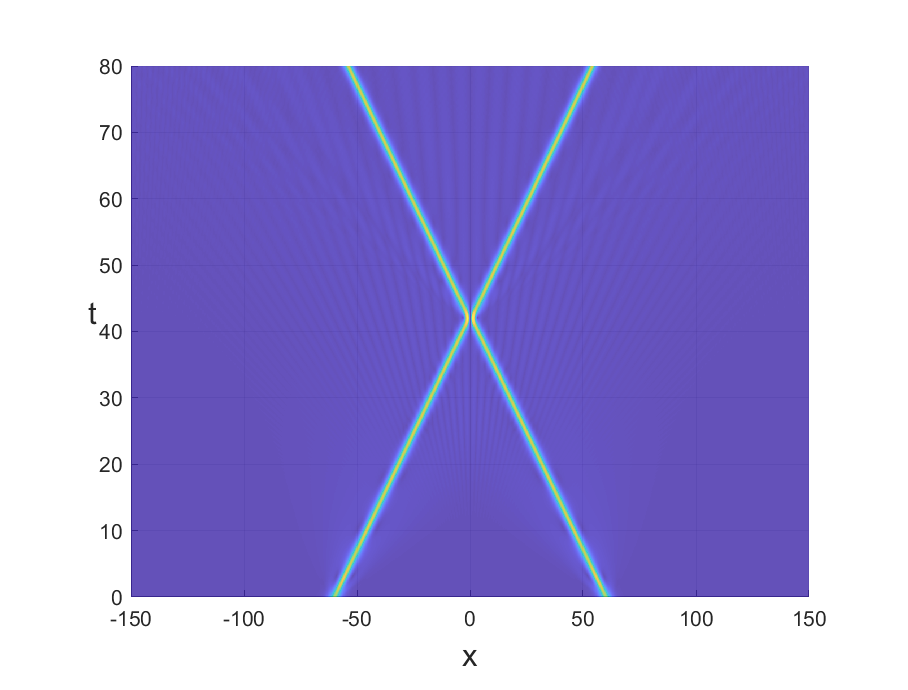
\includegraphics[width=1\linewidth]{fig60.eps}
\subcaption{\(\Delta \theta=\pi,\)\\\( \varepsilon_{2}=0.6,\,\varepsilon_{3}=-0.3\)}
\end{minipage}
\caption{The modulus of numerical solution for soliton collisions at \(k_{1}=-k_{2}=0.7,\,\omega_{1}=\omega_{2}=0\).}
\label{fig50}
\end{figure}

\begin{figure}[H]
\begin{minipage}[h]{0.32\linewidth}
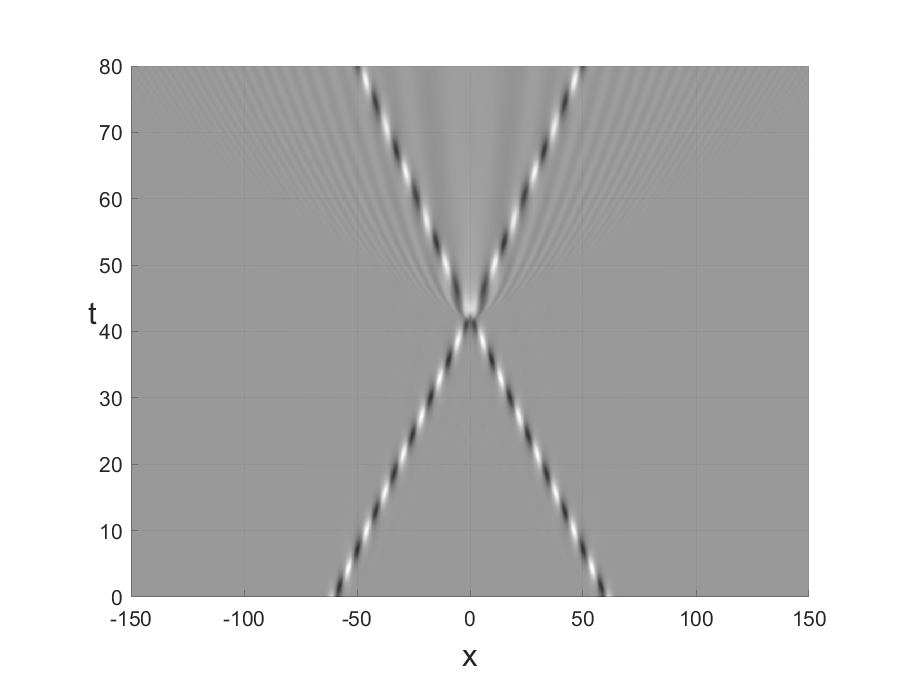
\includegraphics[width=1\linewidth]{fig52g.eps}
\subcaption{\(\Delta \theta=0,\)\\\( \varepsilon_{2}=0.2,\,\varepsilon_{3}=-0.1\)}
\end{minipage}
\begin{minipage}[h]{0.32\linewidth}
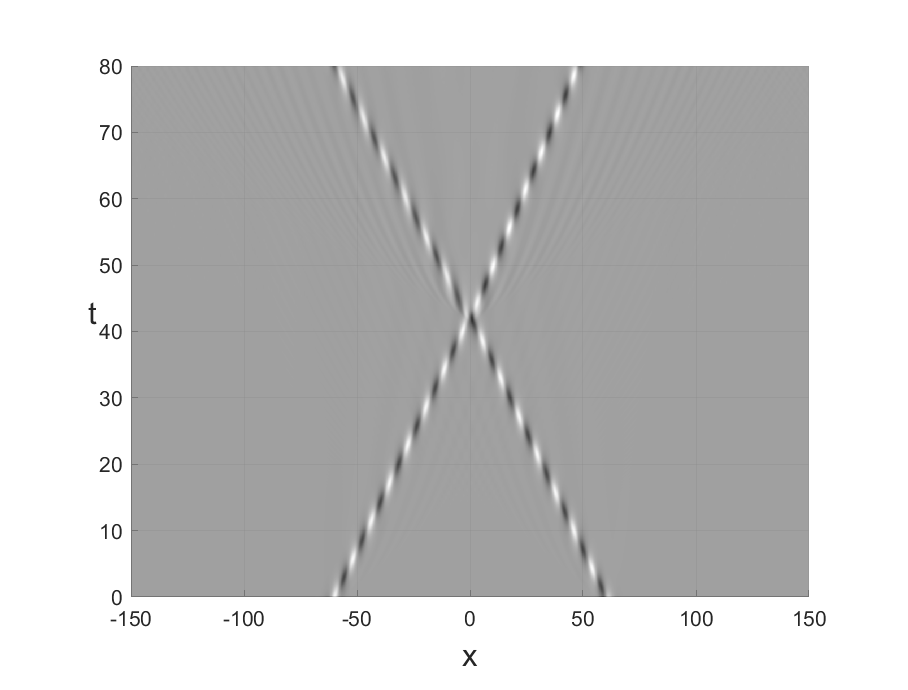
\includegraphics[width=1\linewidth]{fig55g.eps}
\subcaption{\(\Delta \theta=\frac{\pi}{2},\)\\\( \varepsilon_{2}=0.2,\,\varepsilon_{3}=-0.1\)}
\end{minipage}
\begin{minipage}[h]{0.32\linewidth}
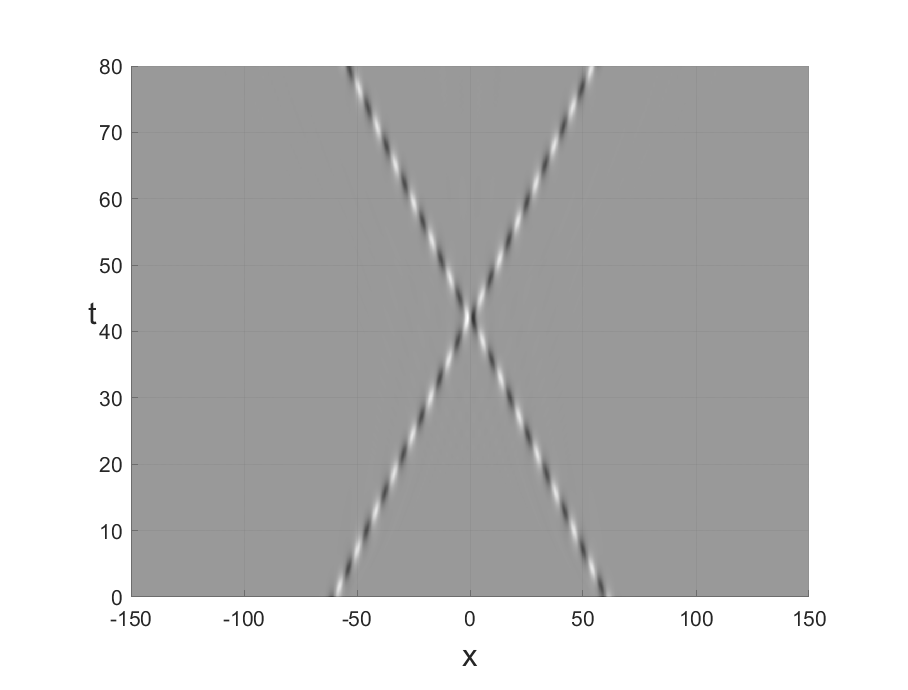
\includegraphics[width=1\linewidth]{fig58g.eps}
\subcaption{\(\Delta \theta=\pi,\)\\\( \varepsilon_{2}=0.2,\,\varepsilon_{3}=-0.1\)}
\end{minipage}

\begin{minipage}[h]{0.32\linewidth}
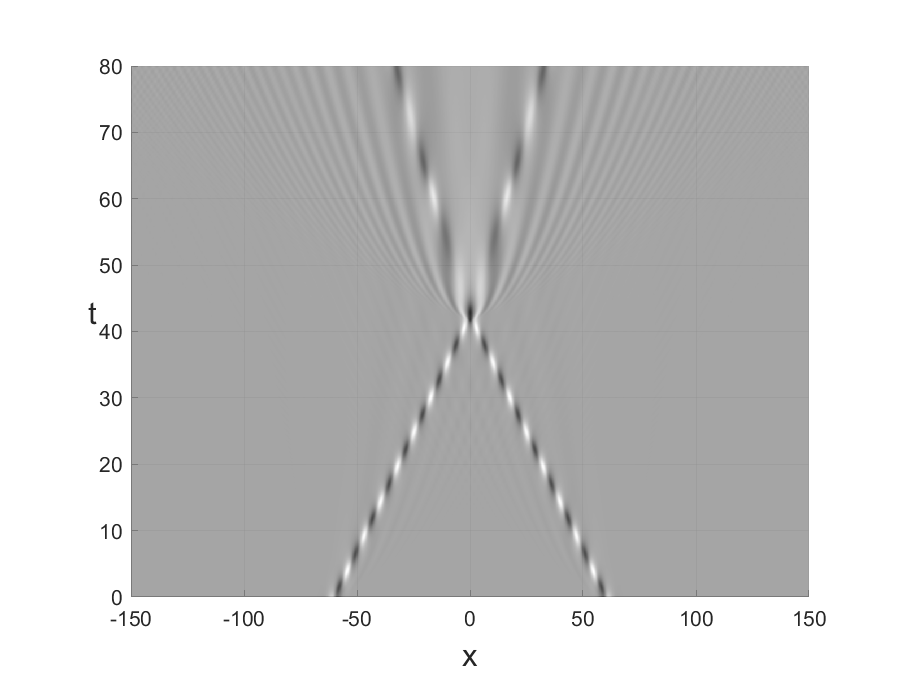
\includegraphics[width=1\linewidth]{fig53g.eps}
\subcaption{\(\Delta \theta=0,\)\\\( \varepsilon_{2}=0.4,\,\varepsilon_{3}=-0.2\)}
\end{minipage}
\begin{minipage}[h]{0.32\linewidth}
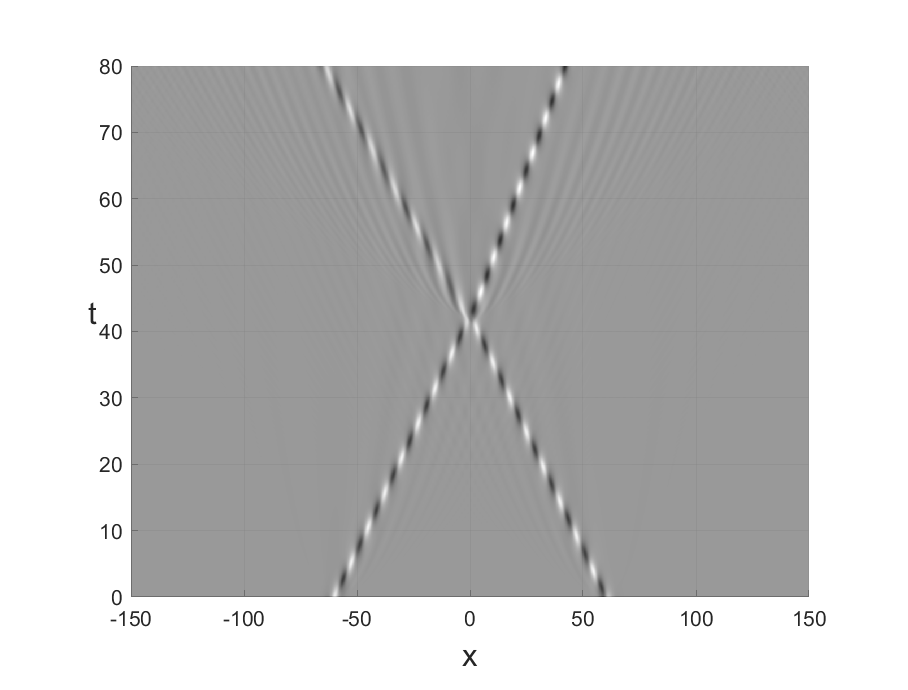
\includegraphics[width=1\linewidth]{fig56g.eps}
\subcaption{\(\Delta \theta=\frac{\pi}{2},\)\\\( \varepsilon_{2}=0.4,\,\varepsilon_{3}=-0.2\)}
\end{minipage}
\begin{minipage}[h]{0.32\linewidth}
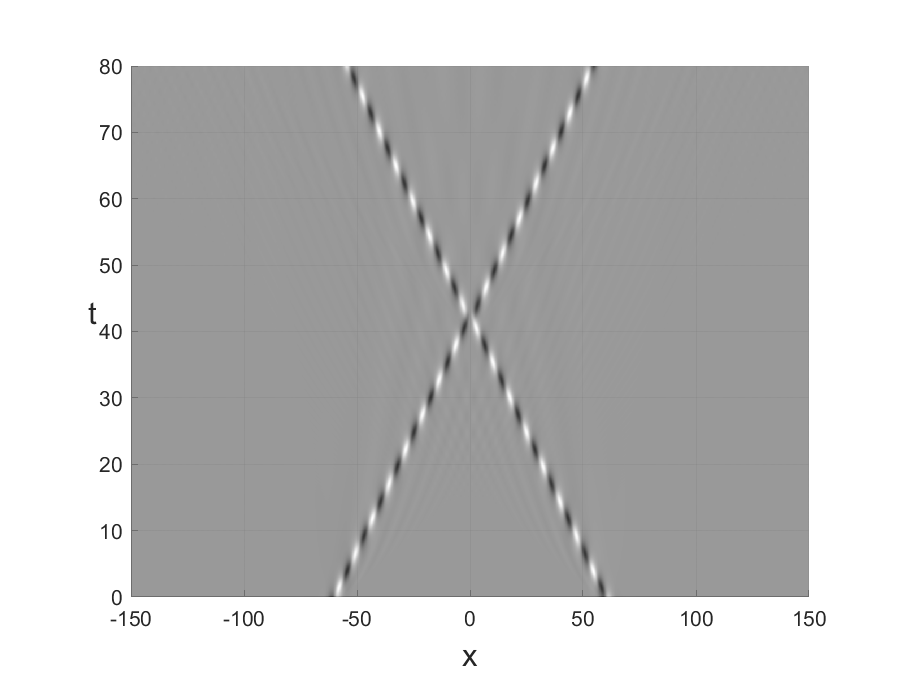
\includegraphics[width=1\linewidth]{fig59g.eps}
\subcaption{\(\Delta \theta=\pi,\)\\\( \varepsilon_{2}=0.4,\,\varepsilon_{3}=-0.2\)}
\end{minipage}

\begin{minipage}[h]{0.32\linewidth}
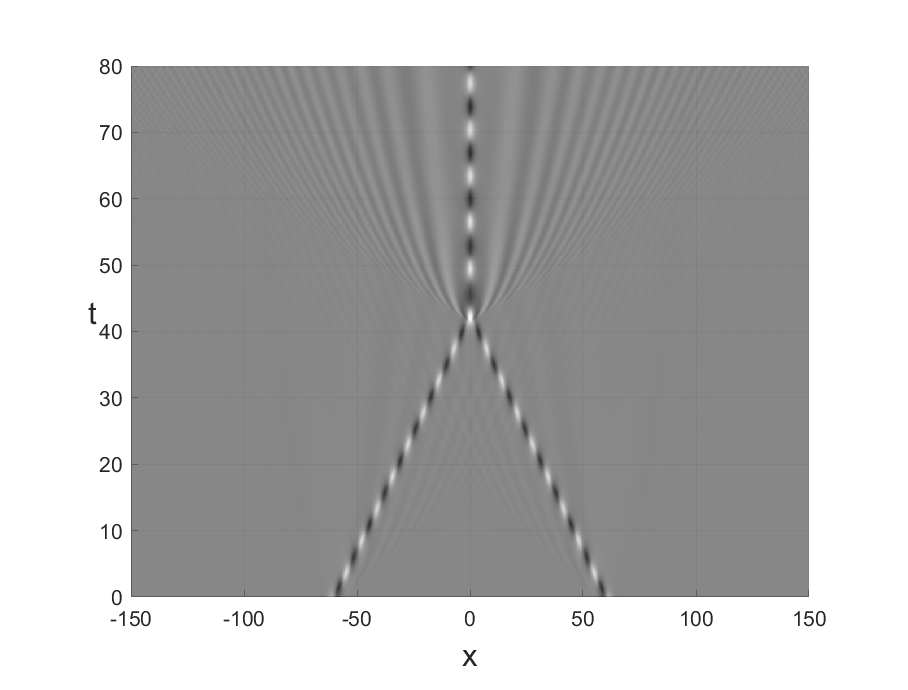
\includegraphics[width=1\linewidth]{fig54g.eps}
\subcaption{\(\Delta \theta=0,\)\\\( \varepsilon_{2}=0.6,\,\varepsilon_{3}=-0.3\)}
\end{minipage}
\begin{minipage}[h]{0.32\linewidth}
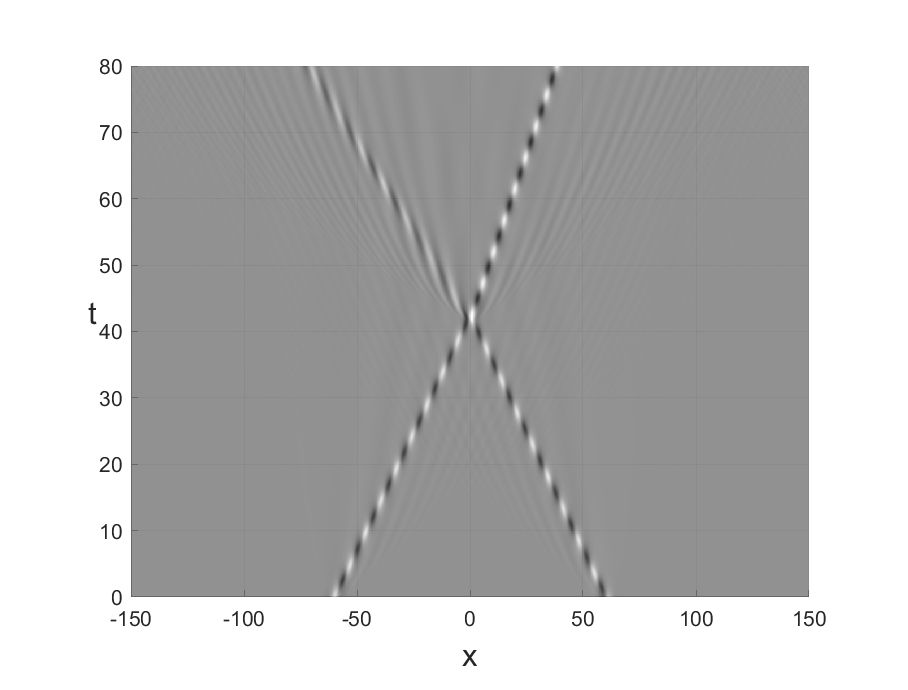
\includegraphics[width=1\linewidth]{fig57g.eps}
\subcaption{\(\Delta \theta=\frac{\pi}{2},\)\\\( \varepsilon_{2}=0.6,\,\varepsilon_{3}=-0.3\)}
\end{minipage}
\begin{minipage}[h]{0.32\linewidth}
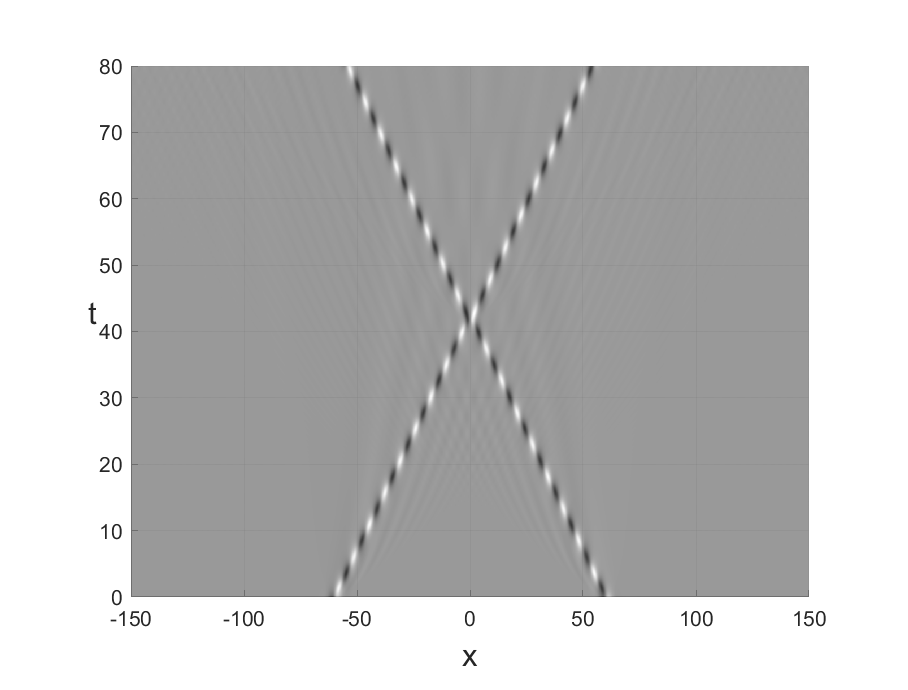
\includegraphics[width=1\linewidth]{fig60g.eps}
\subcaption{\(\Delta \theta=\pi,\)\\\( \varepsilon_{2}=0.6,\,\varepsilon_{3}=-0.3\)}
\end{minipage}
\caption{The real part of numerical solution for soliton collisions at \(k_{1}=-k_{2}=0.7,\,\omega_{1}=\omega_{2}=0\).}
\label{fig51}
\end{figure}

The simulation results allow us to conclude that collisions of solitons in the presence of higher nonlinearity terms can be essentially inelastic. In addition to the perturbation parameters, the certain type of interaction is affected by the difference in the initial phases of the solitons. Near \(\Delta \theta=\pi\), the solitons interact the least intensively. When the phase detuning is in the vicinity of zero, there is a significant energy emission. In this case, there exist a critical perturbation parameters at which two solitons merge into one stationary one. When the parameter \(\Delta \theta \in (0,\,\pi)\), the interaction of solitons occurs with the exchange of energy and momentum.

\section{Conclusions}\label{ch11}
In this paper, we have considered the numerical modeling of the pulse propagation process in a nonlinear medium with periodic boundary conditions described by the cubic-quintic-septic nonlinear Schr\"{o}dinger equation (\ref{eq2}). We have obtained the analytical solution in the form of a solitary wave (\ref{eq24}) and the conditions of its existance. We have modified the split-step Fourier method for modeling pulse propagation processes. We have numerically studied the pulse propogation process and proved the correctness of analytical calculations. We have simulated the interaction of an optical soliton of Eq. (\ref{eq2}) with a perturbation in the initial condition. We have simulated the pulse propogation process in a medium with a random noise. We analyzed the influence of the higher nonlinearity powers to the NLS equation solitary waves propogation. We have simulated the soliton collisions with a presence of highest nonlinear terms.

The following findings are observed from the simulation results:
\begin{enumerate}
  \setlength\itemsep{1em}
  \item The solitary waves of the cubic-quintic-septic nonlinear Schr\"{o}dinger equation propagate steadily.
  \item The optical soliton of the cubic-quintic-septic nonlinear Schr\"{o}dinger equation is not destryed after interaction with disturbance. The pulse is stable when propagating in noisy conditions
  \item Taking into account the higher degrees of nonlinearity, the solitons of the NLS equation transform into a stable soliton solutions of a generalized non-integrable model.
  \item Under conditions of higher nonlinear terms, solitons interact inelastically upon collision. With the addition of the 7th nonlinearity power, the merging of two solitons is possible.

\end{enumerate}

\section*{Acknowledgments}
This research was supported by Russian Science Foundation Grant No. 23-41-00070, https://rscf.ru/en/project/23-41-00070/.
\section*{CONFLICT OF INTEREST}
The authors declare that they have no conflicts of interest.
\section*{ORCID}
Viktor A. Medvedev https://orcid.org/0000-0003-1198-4474\\
Nikolay A. Kudryashov https://orcid.org/0000-0001-5926-9715
%==============================================
%\nocite{*}% Show all bib entries - both cited and uncited; comment this line to view only cited bib entries;

\bibliographystyle{unsrt}
\bibliography{export}

\end{document}
